%------------------------------------------------------------------------------
% Template file for the submission of papers to IUCr journals in LaTeX2e
% using the iucr document class
% Copyright 1999-2013 International Union of Crystallography
% Version 1.6 (28 March 2013)
%------------------------------------------------------------------------------

\documentclass[preprint]{iucr}              % DO NOT DELETE THIS LINE
\usepackage{bm}
% \usepackage{graphicx}
% \usepackage{tabularx}
% \usepackage{subfigure}
% \usepackage{afterpage}
% \usepackage{sansmath}
\usepackage{mathtools}
% \usepackage{parskip}
% \usepackage{tikz}
% \usepackage{tikzorbital}
% \usepackage{setspace}
% \usepackage{xcolor}
\usepackage{amssymb}
% \usepackage{bm}
\usepackage{amsmath}
% \usepackage{fancyhdr}
% \usepackage{rotating}
\usepackage{siunitx}
\usepackage[hyphens,spaces,obeyspaces]{url}
\usepackage{color}
\usepackage{siunitx}
\usepackage[hyphens,spaces,obeyspaces]{url}
\usepackage{color}
%\usepackage{cprotect}
\usepackage{textgreek}
\usepackage[normalem]{ulem}
\usepackage{makecell}

\newcommand{\todo}[1]{{\color{red}[TODO: "#1'']}}
\newcommand{\inblue}[1]{{\color{blue}#1}}
\newcommand{\inred}[1]{{\color{red}#1}}
\newcommand{\ingreen}[1]{{\color{green}#1}}



     %-------------------------------------------------------------------------
     % Infobrmation about journal to which submitted
     %-------------------------------------------------------------------------
     \journalcode{S}              % Indicate the journal to which submitted
                                  %   A - Acta Crystallographica Section A
                                  %   B - Acta Crystallographica Section B
                                  %   C - Acta Crystallographica Section C
                                  %   D - Acta Crystallographica Section D
                                  %   E - Acta Crystallographica Section E
                                  %   F - Acta Crystallographica Section F
                                  %   J - Journal of Applied Crystallography
                                  %   M - IUCrJ
                                  %   S - Journal of Synchrotron Radiation

\begin{document}                  % DO NOT DELETE THIS LINE

     %-------------------------------------------------------------------------
     % The introductory (header) part of the paper
     %-------------------------------------------------------------------------

     % The title of the paper. Use \shorttitle to indicate an abbreviated title
     % for use in running heads (you will need to uncomment it).

\title{X-ray focusing by bent crystals: focal positions as predicted by the crystal lens equation and the dynamical diffraction theory}
% * <msanchezdelrio@gmail.com> 2018-09-25T09:38:50.716Z:
%
% ^.
%\shorttitle{Short Title}

     % Authors' names and addresses. Use \cauthor for the main (contact) author.
     % Use \author for all other authors. Use \aff for authors' affiliations.
     % Use lower-case letters in square brackets to link authors to their
     % affiliations; if there is only one affiliation address, remove the [a].

\cauthor[a]{Jean-Pierre}{Guigay}{guigay@esrf.eu}{address if different from \aff}
\author[a]{Manuel}{Sanchez del Rio}


\aff[a]{European Synchrotron Radiation Facility, 71 Avenue des Martyrs F-38000 Grenoble \country{France}}


     % Use \shortauthor to indicate an abbreviated author list for use in
     % running heads (you will need to uncomment it).

%\shortauthor{Soape, Author and Doe}

     % Use \vita if required to give biographical details (for authors of
     % invited review papers only). Uncomment it.

%\vita{Author's biography}

     % Keywords (required for Journal of Synchrotron Radiation only)
     % Use the \keyword macro for each word or phrase, e.g. 
     % \keyword{X-ray diffraction}\keyword{muscle}

%\keyword{keyword}

     % PDB and NDB reference codes for structures referenced in the article and
     % deposited with the Protein Data Bank and Nucleic Acids Database (Acta
     % Crystallographica Section D). Repeat for each separate structure e.g
     % \PDBref[dethiobiotin synthetase]{1byi} \NDBref[d(G$_4$CGC$_4$)]{ad0002}

%\PDBref[optional name]{refcode}
%\NDBref[optional name]{refcode}

\maketitle                        % DO NOT DELETE THIS LINE

\begin{synopsis}
A crystal lens equation is deduced to address the location of the focus when monochromatic x-ray radiation encounters a bent crystal. It is extended using dynamical theory of diffraction for Laue symmetrical diffraction. Combination of polychromatic and monochromatioc focusing is also discussed. 
\end{synopsis}

%\today
% \begin{flushright}
% {Dedicated to the memory of Claudio Ferrero}
% \end{flushright}

\begin{abstract}
The location of the beam focus  when monochromatic x-ray radiation is diffracted by a \inred{thin} bent crystal is predicted by \inred{a ``}crystal lens equation". We derive this equation \inred{in a general form valid for Bragg and Laue geometries}. This equation has little utility for diffraction in Laue geometry. The \inred{focusing effect in} the Laue symmetrical case is discussed using concepts of dynamical theory and an extension of the lens equation is proposed. The existence of polychromatic \inred{focusing is considered} and the feasibility of matching \inred{the } polychromatic and monochromatic \inred{focal positions} is discussed.   \\

\begin{flushright}
{Dedicated to the memory of Claudio Ferrero}
\end{flushright}

\end{abstract}


     %-------------------------------------------------------------------------
     % The main body of the paper
     %-------------------------------------------------------------------------
     % Now enter the text of the document in multiple \section's, \subsection's
     % and \subsubsection's as required.

\section{Introduction}

The use of curved crystals to diffract and focus x-rays \inred{comes as} a natural extension of the mirror and grating technology for radiation of longer wavelength. Some fundamental concepts, like the Rowland circle, date back to the 19$^\text{th}$ century \cite{rowland1882}.

The fundamental setups using bent crystals to focus X-rays were proposed in the early 1930’s. Some systems use meridional focusing (in the diffraction plane), like i) Johann spectrometer \cite{Johann1931}, \inred{using} a cylindrically bent crystal,  ii) Johansson spectrometer \cite{Johansson1933} \inred{using} a ground and cylindrically bent crystal and iii) the Cauchois spectrometer \cite{cauchois1933} in transmission (Laue) geometry. The von Hamos spectrometer \cite{V.Hamos1933} applies sagittal focusing in the plane perpendicular to the diffraction plane.

With the advent of synchrotron radiation, the concepts of ``geometrical focusing" were applied to design instruments such as polychromators for energy-dispersive extended x-ray absorption fine structure (EXAFS) \cite{Tolentino:ms0206}, monochromators with sagittal focusing for bending magnet beamlines \cite{Sparks1980}, or several types of crystal analyzers \inred{used} at inelastic x-ray scattering beamlines. Bent crystals in transmission or Laue geometry are often employed in beamlines operating at high photon energies. The crystal curvature is used for focusing or collimating the beam in the meridional \cite{Suortti1988,SuorttiShulze} or sagittal \cite{Zhong2001} plane, or just to enlarge the energy bandwidth and improve the luminosity. The crystal bandwidth was optimized and aberrations reduced thanks to \inred{the high collimation and small source size} of synchrotron beams. Curved crystal monochromators work \inred{in} off-Rowland condition, whereas crystal analysers for inelastic scattering studies \inred{work in} the Rowland setting.

% \todo{ REMOVE: The geometrical optics theory is applied for understanding the image formation produced by grazing incidence spherical reflectors \cite{KB1948}. The Gaussian mirror equation (mirror or lens equation), relates the object distance $p$ and the image distance $q$ to the focal length $f$, $p^{-1}+q^{-1}=f^{-1}$, with $f=R_c \sin\theta_B / 2$, where $R_c$ is the mirror curvature radius and $\theta_B$ the Bragg (grazing incidence) angle. However, this mirror or lens equation has limited applications when using crystals, as it can only be applied for symmetric Bragg reflections.}

% The conservation of the tangential component of the wavevector on the crystal surface leads to more general equations in Bragg or Laue geometries, resembling the focusing equations for reflection or transmission gratings.

A ``Crystal Lens Equation" (CLE) was indeed formulated by \cite{CK} for the focusing properties of a cylindrically bent crystal plate diffracting monochromatic x-rays or neutrons, in Laue (transmission) or Bragg (reflection) geometries. The crystal is bent around an axis perpendicular to the diffraction plane (meridional focusing). This CLE is based on a purely geometric approach in which multiple \inred{Bragg} scattering (dynamical effects) \inred{is neglected}. 
The CLE is \inred{revisited} in Section~\ref{sec:CLE}, \inred{in order to correct errors} found in \cite{CK} for the Laue geometry. \inred{A new formula valid in Bragg and Laue geometry is obtained, using the same geometrical approach as in \cite{CK}}.

The CLE has wide applicability in Bragg geometry. However, \inred{its use for Laue geometry} is \inred{limited to very thin crystals, because
it ignores} a \inred{basic} dynamical focusing effect \inred{also found in flat crystals},
as described in section~\ref{sec:dynamlicalLaue}. 
The \inred{applicability} of the lens equation in symmetrical Bragg geometry is discussed in \inred{appendix}~\ref{sec:BraggGeometry}. %with comparison to recent numerical simulations \cite{Honkanen2018}) which are based on a finite element method to take the propagation in the crystal into account.
The CLE concerns the focusing of monochromatic radiation, and is in general different from the condition of polychromatic focusing. The particular cases where these two different focusing conditions coincide are discussed in section~\ref{sec:polychromatic}. A final summary is given in section~\ref{sec:summary}.   


\section{The crystal lens equation revisited}
\label{sec:CLE}

\inred{The lens equation will be derived in Bragg or Laue geometry, with source $S$ and focus $F$ in real or virtual position (see Fig.~\ref{fig:geometries}).} Consider a monochromatic x-ray or neutron beam \inred{from a real or virtual} point-source $S$. The origin of coordinates $O$ is chosen at the point of the crystal surface in such a way that the wave-vector  ${\vec k_0}$ of the incident ray $\overline{SO}$ is in exact Bragg  position. The \inred{wave-vector of the} diffracted ray \inred{in vacuum is } 
% $\vec k_h$ given by the Laue equation 
$\vec k_h = \vec k_0 + \vec h$, where $\vec h$ is the reciprocal lattice vector (see Fig.~\ref{fig:vectors}).
\inred{in} both transmission geometry (Laue) or reflection geometry (Bragg).
% \inred{and the vectors $\vec k_h$, $\vec k_0$ and $\vec h$ are in vacuum}. 

\begin{figure}
\label{fig:geometries}
\caption{Schematic representation of the different diffraction setups with real or virtual source in Bragg or Laue \inred{cases}:
a) real source, real focus (red) in Laue case \inred{or} virtual focus (blue) in Bragg case,
b) real source, virtual focus (red) in Laue case \inred{or} real focus (blue) in Bragg case,
c) virtual source, real focus (red) in Laue case \inred{or} virtual focus (blue) in Bragg case,  
d) virtual source, virtual focus (red) in Laue case \inred{or} real focus (blue) in Bragg case.
\inred{$L_0=\overline{SO}$ is the distance source to crystal and $L_h=\overline{OF}$ is the distance crystal to focus.}
}
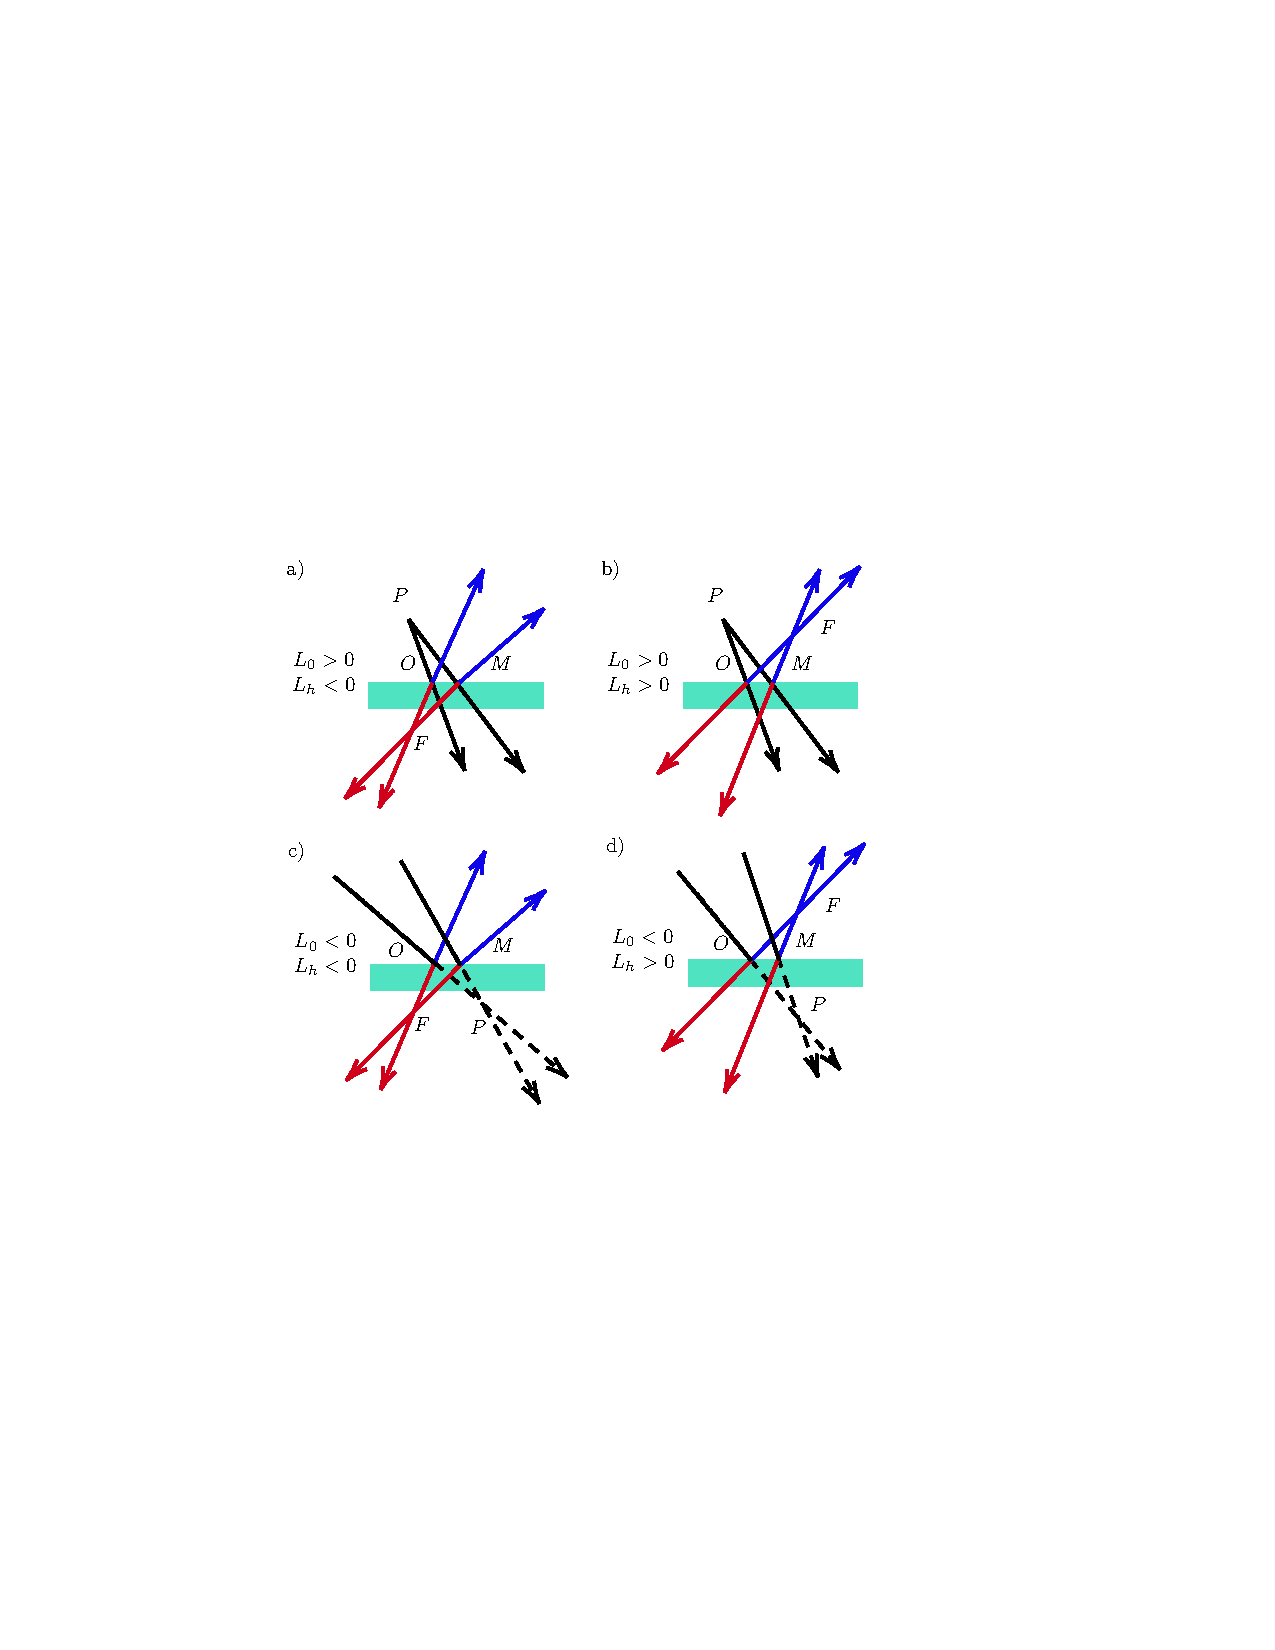
\includegraphics[width=0.99\textwidth,trim=4cm 9cm 6cm 9cm,clip=true]{fig1.pdf}
\end{figure}


\inred{The inward normal to the crystal surface in $O$ is $\vec n$, and $\varphi_0 = (\vec n, \vec k_0)$ is the oriented angle from the vector $\vec n$ to the vector $\vec k_0$. Similarly,} $\varphi_h = (\vec n, \vec k_h)$. Without loss of generality $\varphi_0$ is positive; $\theta_B$ is the Bragg angle \inred{(always positive)}.
\inred{In the}  case of symmetric geometry(asymmetry angle $\alpha=0$) \inred{we find} $\varphi_{0,h}=\pm\theta_B$ in Laue or $\varphi_{0,h}=(\pi/2)\mp\theta_B$ in Bragg. Otherwise, the asymmetry angle $\alpha$ is defined as the angle of rotation \inred{of the vector $\vec h$ from its direction in the symmetrical case}. 
% It follows that $\varphi_0+\varphi_h=2\alpha$ in Laue case and  $\varphi_0+\varphi_h=2\alpha+\pi$ in Bragg case.
In Laue case $\varphi_{0,h}=\pm\theta_B+\alpha$; in Bragg case $\varphi_{0,h}=(\pi/2)\mp\theta_B+\alpha$, therefore $2\theta_B=|\varphi_0-\varphi_h|$ in both cases, $2\alpha=\varphi_0+\varphi_h$ in Laue case and $2\alpha=\varphi_0+\varphi_h-\pi$ in Bragg case.


When moving the point of incidence over an arbitrary small distance $s$ along the curved crystal surface (see Fig.~\ref{fig:vectors}), 
$\vec k_{0,h}$ are changed
% in direction (not in modulus), 
with rotation angles $\epsilon_{0,h} = (\vec k_{0,h},\vec k'_{0,h})$; $\vec h$ and $\vec n$ are changed into $\vec h'$ and $\vec n'$, respectively, due to the crystal bending;
$\varphi_{0,h}$ are changed into $\varphi'_{0,h}=\varphi_{0,h}+\Delta \varphi_{0,h}$.
The projections of the vectors $\vec k'_{h}$ and $\vec k'_{0}+\vec h'$ on the crystal surface are equal \inred{(}conservation of the parallel components of wave-vectors\inred{)}.
% The surface projection of $\vec k'_{0,h}$ are equal to $k \sin\varphi'_{0,h}$.
Furthermore, in the present case of cylindrical bending \inred{of very thin crystal}, the surface projection of $\vec h'$ is constant (the angle between $\vec h$ and $\vec n$ is constant).
This implies that $(\sin \varphi_h - \sin \varphi_0)$ is invariant, therefore
\begin{equation}
\label{eq:invariant}
    \Delta \varphi_h \cos\varphi_h = \Delta \varphi_0 \cos\varphi_0.
\end{equation}

\begin{figure}
\label{fig:vectors}
\caption{Schematic view of the relevant parameters in focusing by a bent crystal in Bragg geometry.
}
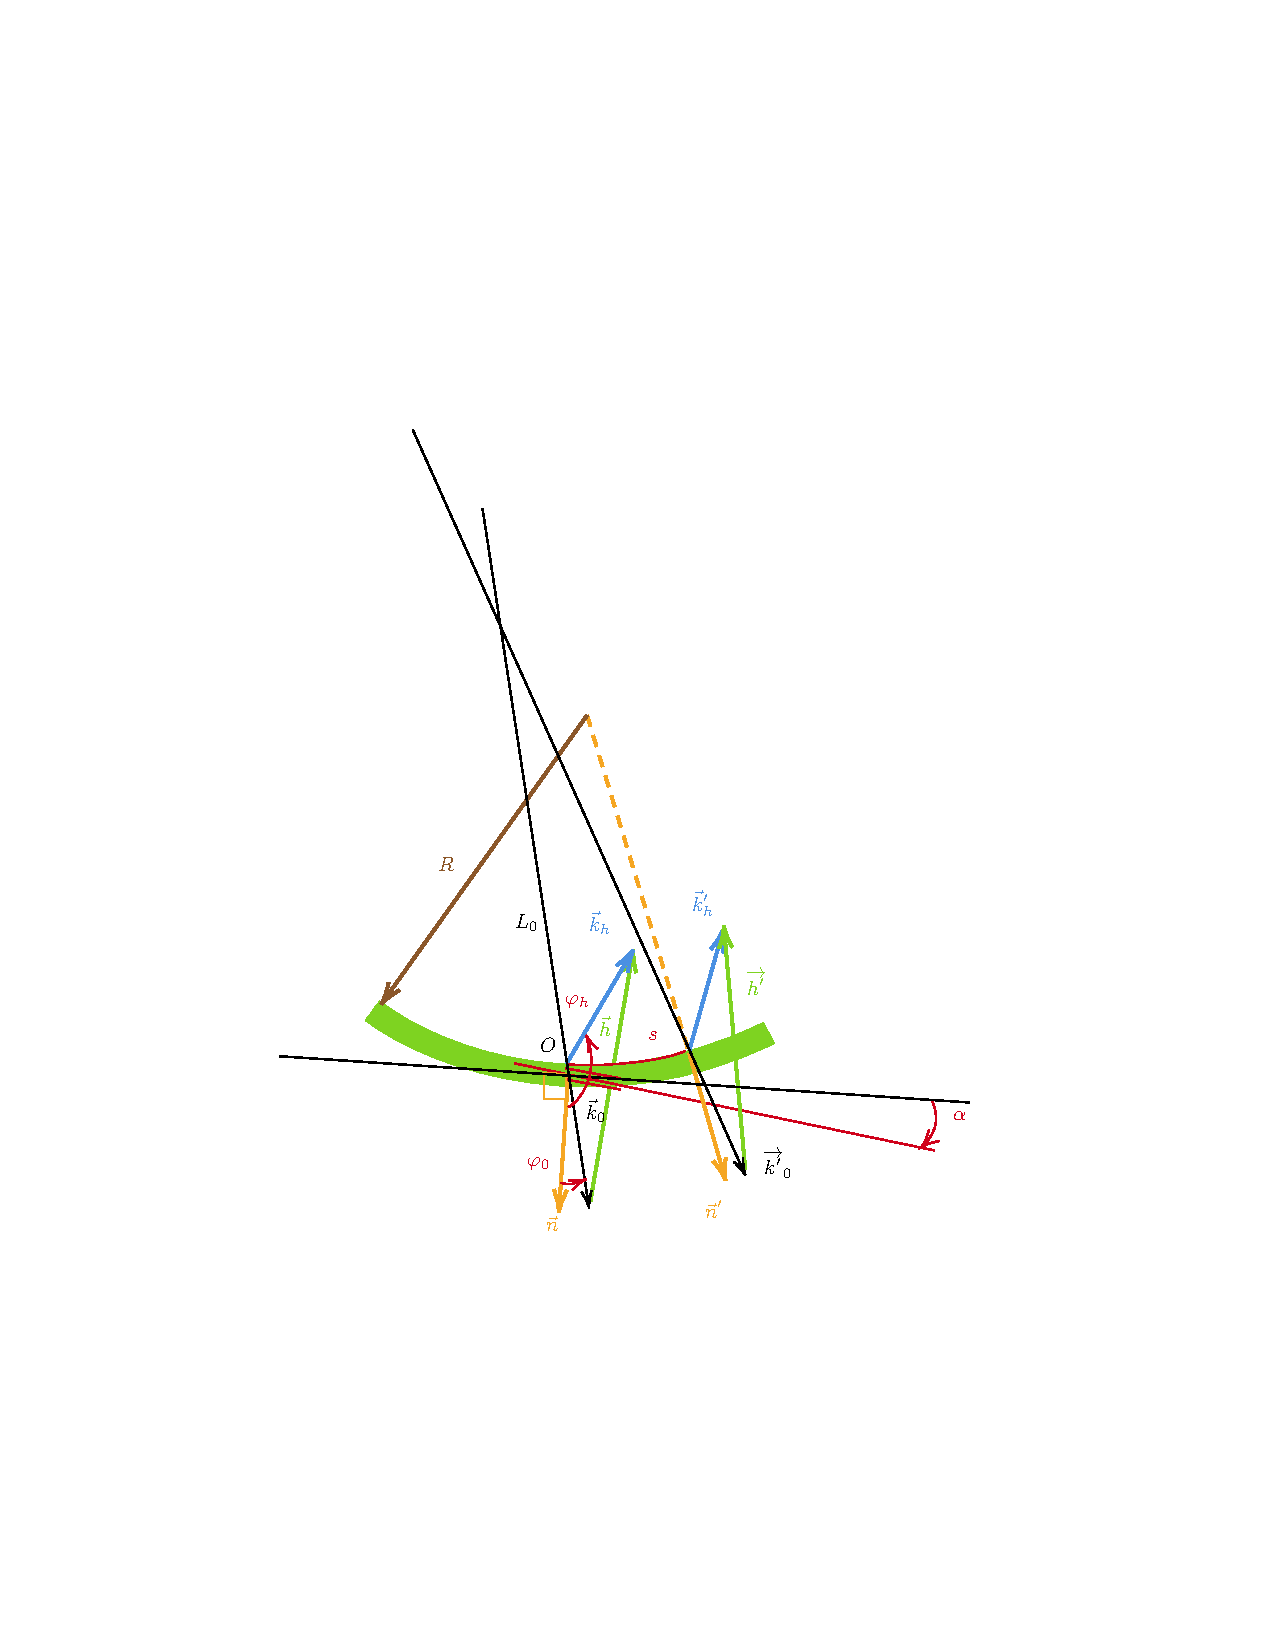
\includegraphics[width=0.99\textwidth,trim=4cm 6cm 5cm 10cm,clip=true]{fig2.pdf}
\end{figure}

The source distance $L_0=\overline{SO}$ is set as positive if the source is on the incidence side of the crystal (real source) or negative if the source is on the other side (virtual source) (see Fig.~\ref{fig:geometries}). The radius of curvature $R_c$ is set as positive if the beam is incident on the concave side of the bent crystal. The focus distance $L_h$ is set as positive if the \inred{(}real or virtual\inred{)} focus \inred{$F$} is situated on the incidence side on the crystal. With these conventions, $(\vec n,\vec n')=s/R_c$, $\epsilon_0 L_0 = s \cos\varphi_0$,  $\epsilon_h L_h = s |\cos\varphi_h|$. Using the relationship
\begin{equation}
    \varphi'_{0,h} = 
    (n',  \vec k'_{0,h}) = 
    (\vec n', \vec n) + (\vec n,\vec k_{0,h}) + (\vec k_{0,h}, \vec k'_{0,h}) = -\frac{s}{R_c} + \varphi_{0,h} + \epsilon_{0,h},
\end{equation}
we obtain
% \footnote{\inred{Equation~(\ref{eq:angles}) here has a different global sign than the corresponding (wrong) equation (9) in \cite{CK} }}
\begin{equation}
\label{eq:angles}
\Delta \varphi_0 =  - \frac{s}{R_c} + s \frac{\cos\varphi_0}{L_0}
\end{equation}
and 
\begin{equation}
\label{eq:angles2}
\Delta \varphi_h = - \frac{s}{R_c} +  s \frac{|\cos\varphi_h|}{L_h}.
\end{equation}

The crystal lens equation \inred{valid in both Bragg and Laue cases,} is finally obtained by inserting these expressions in equation~(\ref{eq:invariant})

\begin{equation}
\label{eq:CLE}
\frac{|\cos\varphi_h| \cos\varphi_h}{L_h} - \frac{\cos^2\varphi_0}{L_0} = \frac{\cos\varphi_h - \cos\varphi_0}{R_c}.
\end{equation}


% Equation~\ref{eq:CLE} is valid in both Bragg and Laue cases.
In the Laue symmetrical case ($\cos\varphi_h=\cos\varphi_0$) it predicts $L_h=L_0$ (for a real source, the focus is virtual at the same distance as the source) and, in the particular case of $L_0=+\infty$, a plane incident wave is diffracted into a plane wave.

The crystal lens equation~(\ref{eq:CLE}) obtained here is different from the equation given in \cite{CK}\footnote{The CLE \inred{given} in \cite{CK} is 
\inred{$
\cos^2\varphi_0/L_0 + \cos^2\varphi_h/L_h = (\cos\varphi_0 + |\cos\varphi_h|)/R_c$}.
We think this is due to mistakes in their calculations, specially sign errors in their equation (9) as compared \inred{to} our equation~(\ref{eq:angles}). 
}.
Both equations are equivalent for the Bragg case ($\cos\varphi_h<0$)\inred{, which is also considered by \citeasnoun{snigirevkohn1995}.} They are not equivalent in the Laue case.
 
% It is worth mentioning that the lens equation~(\ref{eq:CLE}) discussed here can be applied only for monochromatic radiation. Polychromatic focusing is discussed in section~\ref{sec:polychromatic} in the more general context of dynamical theory of diffraction.
Note that we used in this section the same notation as \cite{CK}, where $R_c$ is positive for a concave surface, used to focus in Bragg case. For the rest of the paper, we \inred{also use} the notation: $p \leftarrow L_0$, $q \leftarrow -L_h$ $R \leftarrow -R_c$, $\theta_1 \leftarrow \varphi_0$ and $\theta_2 \leftarrow \varphi_h$\inred{, which is more convenient} for Laue crystals, because real focusing is obtained when the beam coming from a real source is incident on the convex side of the bent crystal (with positive $R$).

Equation~(\ref{eq:CLE}) is obtained here using a geometrical ray optics approach. It can also be deduced from a wave-optics approach as shown in Appendix~\ref{appendix:CLE}.

\section{Dynamical focusing in Laue geometry}
\label{sec:dynamlicalLaue}

The \inred{applicability} of the CLE for the Laue case is \inred{limited to very thin crystals}. The dynamical theory \inred{(see book \cite{authierbook})}
% of diffraction 
predicts ``new" focal conditions, even for flat Laue crystals.
% that are relevant in experiments and are not explained by the simple CLE. 
\inred{This is} analyzed here in the framework of the \inref{Takagi-Taupin equations, hereafter TTE} \inred{\cite{Takagi1962, Takagi, Taupin, Taupin1967}}. 


\inred{
Section~\ref{sec:influence} deals with the derivation of the ``influence functions" (Green functions) which represent the wavefield generated in the crystal by a point-source on the crystal entrance surface.

In section~\ref{sec:LaueFlat}, the approach to dynamical focusing in the symmetric Laue case
\cite{kushnir, GuigayFerrero2013}
% (Kushnir & Suvorov, 1982; Guigay et al, 2013)
is extended to asymmetric geometry. The effects of anomalous absorption (Borrmann effect) are obtained in parallel. The new concept of ``numerically determined focal length" of a flat crystal, denoted as $q_{dyn}$, is introduced.

In section~\ref{sec:LaueNewCLE}, a lens equation for a bent Laue symmetrical crystal of finite thckness, expressed in terms of $q_{dyn}$ is established. Its predictions are shown to be in agreement with numerical calculations. 

In section~\ref{sec:LaueCompatibilityCLE}, we make the verification that the formulation for the Laue asymmetric case by
% (Guigay & Ferrero , 2016) 
\cite{GuigayFerrero2016} is in agreement with the CLE (equation (\ref{eq:CLE})) in the limit of vanishing crystal thickness.}
% \inblue{Here, after introducing basic results from the Takagi-Taupin equations in section~\ref{sec:influence}, we give a simple description of the \inred{basic} focusing effect in the case of a flat crystal plate of finite thickness (section \ref{sec:LaueFlat}). Then, we deduce in section~\ref{sec:LaueNewCLE} an improved form of the CLE for a Laue bent crystal (presently, only in the case of symmetric reflection). We verified its convergence to the CLE in the limit of vanishing crystal thickness (section~\ref{sec:LaueCompatibilityCLE}). }

\subsection{Influence function derived from Takagi-Taupin equations}
\label{sec:influence}

% We introduce the Takagi-Taupin equations and the influence functions representing the wavefield for a point-source on the crystal entrance surface. 
The x-ray wavefield inside the crystal is expressed as the sum of two modulated plane waves
\begin{equation}
    \Psi(\vec x) = D_0(\vec x) e^{i \vec k_0 . \vec x} + D_h(\vec x) e^{i \vec k_h . \vec x},
\end{equation}
with slowly varying amplitudes $D_{0,h}(\vec x)$.
The spatial position $\vec x$ is expressed in oblique coordinates $(s_0,s_h)$ along the directions of the $\vec k_0$ and $\vec k_h=\vec k_0 + \vec h$ vectors\inred{, which are the in-vacuum wave-vectors ok modulus $k=2\pi/\lambda$. $\vec{h}$ is the Bragg diffraction vector of the undeformed crystal. In such conditions,} the differential TTE are
% \cite{Takagi1962, Takagi, Taupin, Taupin1967}, hereafter referred to as TTE, are
\begin{subequations}
\label{eq:TT}
\begin{align}
\frac{\partial D_0}{\partial s_0} =& \frac{ik}{2} \left[ \chi_0 D_0(\vec x)+c \chi_{\bar h} e^{i \vec h . \vec u (\vec x)} D_h(\vec x) \right]; \\
\frac{\partial D_h}{\partial s_h} =& \frac{ik}{2} \left[ \chi_0 D_h(\vec x)+c \chi_{h} e^{-i \vec h . \vec u (\vec x)} D_0(\vec x) \right],
\end{align}
\end{subequations}
where $\chi_0$, $\chi_h$, and $\chi_{\bar h}$ are the Fourier coefficients of order 0, $\vec h$ and $-\vec h$ of the undeformed crystal polarisability. The polarization factor $c$ ($c=1$ for $\sigma$-polarization and $c=\cos2\theta_B$  for $\pi$-polarization) \inred{is} omitted afterwards. 
$\vec u (\vec x)$ is the displacement field of the deformed crystal.
% The ``influence functions", hereafter called IF, are the solutions of the TT equations corresponding to a point source in the crystal entrance surface.
In the case of \inred{cylindrical bending we have}
\begin{equation}
\label{eq:cylinder}
    \vec h . \vec u = -A s_0 s_h + \phi_1(s_0) - \phi_2(s_h)
\end{equation}
where $A$ and the $\phi_{1,2}$ functions are \inred{defined} in Appendix~\ref{appendix:Deformation}.
This a 
% Equation~(\ref{eq:cylinder}) corresponds to the case of a 
``constant strain gradient" \inred{case} \cite{authierbook} meaning that $\partial^2(\vec h . \vec u)/(\partial s_0 \partial s_h)$ is constant. \inred{In terms of} the functions $G_{0,h}(s_0,s_h)$ defined by
\begin{subequations}
    \label{eq:functionsG}
    \begin{align}
      D_0(s_0,s_h) &= G_0(s_0,s_h) \exp[i\frac{k}{2}\chi_0 (s_0+s_h)-i \phi_2(s_h)]\\
      D_h(s_0,s_h) &= G_h(s_0,s_h) \exp[i\frac{k}{2}\chi_0 (s_0+s_h)-i \phi_1(s_0)+iAs_0s_h],
    \end{align}
\end{subequations}
the TTE have a simpler form
\begin{subequations}
    \label{eq:TTEsimple}
    \begin{align}
      \frac{\partial G_0}{\partial s_0} &= i \frac{k}{2}\chi_{\bar{h}} G_h
      \\
      \frac{\partial G_h}{\partial s_h} &= i \frac{k}{2}\chi_{h} G_0 - i A s_0 G_h.
    \end{align}
\end{subequations}

An incident monochromatic wave of any form can be expressed as a modulated plane wave $D_{inc}(\vec x)\exp(i \vec k_0 . \vec x)$ defining a continuous distribution of coherent elementary point-sources on the crystal surface, according to the general Huyghens principle in optics. The “influence functions” \inred{or Green functions}, hereafter IF, are the TTE solutions \inred{for} these point-sources. 
The IF for point-sources of oblique coordinates $(\sigma_0,\sigma_h)$
% , in the case of  a crystal with deformation that fulfills equation~(\ref{eq:cylinder}), 
are derived in \cite{GuigayFerrero2016} by formulating the TTE  as integral equations in the case of an incident \inred{amplitude} of the form \inred{$D_{inc}=\delta(s_h-\sigma_h)$}. 
The calculations (see appendix~\ref{appendix:TTEintegral}) result in the diffracted amplitude\footnote{the result for the transmitted amplitude $D_0(s_0,s_h)$ is not necessary for our results and is not presented here, but it is easily obtained using equation~(\ref{eq:kummer}) in (\ref{eq:TTEsimple}).}

  
\begin{equation}
\label{eq:kummer}
    D_h(s_0,s_h) = \frac{i k }{2} \chi_h e^{(ik/2) \chi_0 (s'_0 + s'_h)} e^{-i \vec h . \vec u (s_0,\sigma_h)} M(\frac{i\Omega}{A},1,iA s'_0 s'_h)
\end{equation}
where the first exponential term stands for the effects of refraction and normal absorption, $s'_{0,h}=s_{0,h}-\sigma_{0,h}$; $\Omega=k^2\chi_h\chi_{\bar{h}}/4$ and the $M$-function is the Kummer function (a confluent hypergeometric function) defined by the convergent infinite series
\begin{equation}
\label{eq:kummerSeries}
    M(a,b,z) = 1 + \frac{a}{b} z + 
    ... + \frac{a(a+1)...(a+n-1)}{n! b (b+1)...(b+n-1)}z^n+...
\end{equation}

This \inred{type of TTE solution} was already obtained by different methods \cite{Petrashen1974,Katagawa1974,Litzmann1974,Chukhovski1977}.

% The exponential term $\exp(i \vec h . \vec u(s_0,\sigma_h))$ in equation~(\ref{eq:kummer}) is the phase shift acquired at the scattering event occurring at the point of oblique coordinates $(s_0,\sigma_h)$along the ray incident in the point $(\sigma_0,\sigma_h)$. It therefore represents the kinematical (single-scattering) approximation of the dynamical theory.
\inred{
It is noticeable that the term $\exp[-i\vec h . \vec u (s_0,\sigma_h)]$ in equation~(\ref{eq:kummer}) is the phase shift acquired by scattering at the point of coordinates $(s_0,\sigma_h)$ along the incident ray. We can say that the kinematical (single-scattering) approximation of equation~(\ref{eq:kummer}) is 

\begin{equation}
\label{eq:kummerapprox}
    D_{h,kin}(s_0,s_h) = \frac{i k }{2} \chi_h e^{(ik/2) \chi_0 (s'_0 + s'_h)} e^{-i \vec h . \vec u (s_0,\sigma_h)} 
\end{equation}
and the full multiple scattering is $D_h=D_{h,kin} M$.
}

% In the case of $A=0$ \inred{(symmetric diffraction)}, the Kummer function in equation~(\ref{eq:kummer}) reduces to the Bessel function $J_0(2\sqrt{\Omega s'_0 s'_h})$. 
          
\subsection{Dynamical focusing and Borrmann effect in a flat\inred{, asymmetric, Laue} crystal}
\label{sec:LaueFlat}



Dynamical focusing \inred{by} flat Laue crystals (without bending) \inred{was predicted by} \citeasnoun{AfanasevKohn1977} and verified experimentally by \cite{Aristov1978,Aristov1980PhysStatSol,Aristov1980}
in the case of symmetrical geometry. The theory was extended to the asymmetric case by \citeasnoun{Kohn2000}. \inred{The application of dynamical focusing to high-resolution spectrometry was proposed by \citeasnoun{KohnGorobtsov2013}.}
% The dynamical diffraction focusing by a system of two Laue crystals was recently considered by \cite{KohnSmirnova}. Diffraction focusing by a system of two identical perfect Laue crystals was previously applied to neutron interferometry \cite{Zeilinger}.

\begin{figure}
\label{fig:laue}
\caption{Schematic representation of the relevant parameters in Laue asymmetrical diffraction.
}
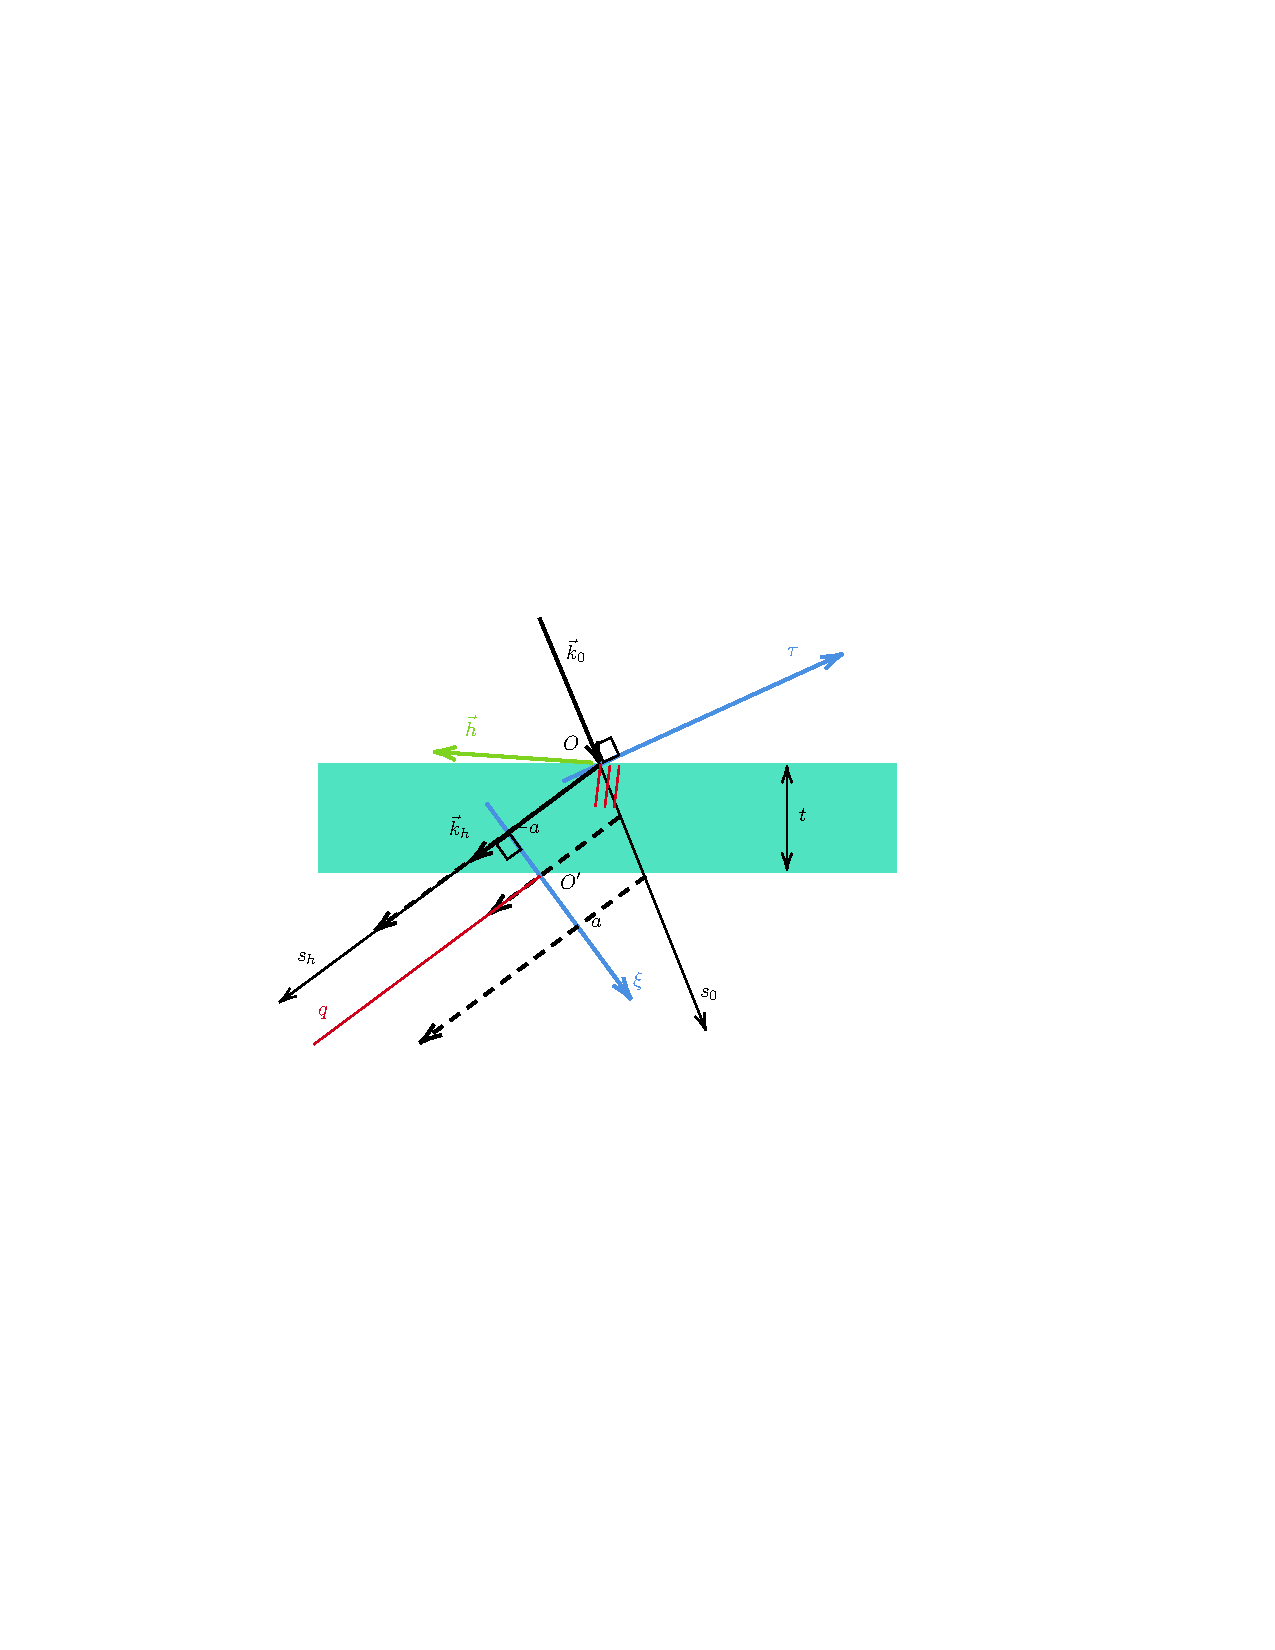
\includegraphics[width=0.99\textwidth,trim=3cm 10cm 5cm 10cm,clip=true]{fig3.pdf}
\end{figure}

% The incident wave-amplitude is expressed in a plane perpendicular to the incidence direction at a negligible distance from the entrance surface (axis $\tau$ in Fig.~\ref{fig:laue}).
% Similarly, we will express the Bragg-diffracted amplitude $D_h$ in a plane perpendicular to the direction of the Bragg diffraction at a negligible distance from the exit surface (axis $\xi$ in Fig.~\ref{fig:laue}). 
% The dynamical focusing is most easily described by considering a point-source on the crystal entrance surface (in practice, a slit of negligible width placed near the crystal surface).

\inred{The basic case of dynamical focusing is that of a point-source in $O$ ($\sigma_0=\sigma_h=0$)} on the crystal entrance surface \inred{of the crystal of thickness $t$}.
% (in practice, a slit of negligible width placed near the crystal surface).
\inred{$O'$ is the middle of the basis of the influence region (Borrmann fan) on the exit surface (see Fig.~\ref{fig:laue}).}
% A point in the $\xi-$axis perpendicular to the direction of $\vec k_h$ and at negligible distance from the crystal of thickness $t$ (see Fig.~\ref{fig:laue}), corresponds to a point of oblique coordinates 
\inred{
The amplitude of the diffracted wave along the axis $O'\xi \perp \vec k_h$ is the value of the IF at the point of coordinates 

\begin{equation}
    \label{eq:s0andsh}
    s_0 = \frac{a+\xi}{\sin2\theta_B }  ; \:\: 
    s_h = \gamma\frac{a-\xi}{\sin2\theta_B},
\end{equation}
}
with $a=t \sin2\theta_B/(2\cos\theta_1)$ and $\gamma=\cos\theta_1/\cos\theta_2$. 



The amplitude $D_h(\xi)$ is zero outside the interval $-a<\xi<a$,
% , with $a=t \sin2\theta_B/(2 \cos\theta_1)$, 
and is proportional to the Bessel function \inred{$J_0(k \sqrt{\chi_h \chi_{\bar h} s_0 s_h})=$} $J_0(Z\sqrt{a^2-\xi^2})$ in this interval \cite{kato1961}, with  $Z=k\sqrt{\gamma\chi_h\chi_{\bar h}}/\sin2\theta_B$. In the case $|Z a| \gg 1$ the asymptotic approximation
\begin{equation}
    J_0(Z\sqrt{a^2-\xi^2})\approx \left(\frac{2}{\pi Z \sqrt{a^2-\xi^2}}\right)^{1/2} \cos(Z\sqrt{a^2-\xi^2}-\pi/4)
\end{equation}
can be used in the central region $|\xi|\ll a$ where \inred{$\sqrt{a^2-\xi^2} \approx a - \frac{\xi^2}{2a}$}.
% \todo{DELETE THIS EQUATION} 
% \begin{equation}
%      \sqrt{a^2-\xi^2} = a (1-\frac{\xi^2}{2a^2}+...)\approx a - \frac{\xi^2}{2a}.
% \end{equation}
We thus obtain in this central region the approximation
\begin{equation}
\label{eq:approximatedDiffractedField}
    J_0(Z\sqrt{a^2-\xi^2})\approx \left(\frac{2}{i \pi Z a}\right)^{1/2} \left( e^{iZa-i Z\frac{ \xi^2}{2a}} + i 
    e^{-i Z a+i Z\frac{\xi^2}{2a}} \right),
\end{equation}
where the two exponential terms are related to the two sheets of the dispersion surface. 
\inred{The} function $\exp(- i Z \xi^2 / (2 a))$ 
represents a converging wave if $\operatorname{Re}(Z)>0$ (divergent if  ($\operatorname{Re} Z <0$). A double, real and virtual, focusing effect is thus expected at opposite distances $\pm q_0$ from the crystal, with
\begin{equation}
\label{eq:q0}
    q_0 = \frac{k a}{|\operatorname{Re}(Z)|}= \frac{a \sin2\theta_B}{|\operatorname{Re}(\sqrt{\gamma\chi_h\chi_{\bar h}})|}
\end{equation}

\inred{This equation is present in \cite{Kohn2000, KohnGorobtsov2013} in a different form and from a different point of view. These authors consider a point-source at a finite distance and their equation determines the value of the crystal thickness needed to focus the diffracted wave on the back crystal surface. A noticeable difference is that our equation is expressed in terms of $\chi_h \chi_{\bar h}$ without approximations  concerning the real and imaginary parts of the crystal polarizability. In the works cited above $\operatorname{Re}} (\sqrt{\chi_h \chi_{\bar h}})$ is approximated by $|\chi_{hr}|$ or $|\chi_h|$.
}

\inred{The moduli of the two terms in equation~(\ref{eq:approximatedDiffractedField}) are proportional to $\exp(\mp a \text{Im}~(Z))$, respectively. This is the expression of anomalous absorption (Borrmann effect). Two focal positions will be observed for small absorption, but only one for strong absorption, as shown in Fig.~\ref{fig:flatLaue}.
}

% The parameter $q_0$, which may be referred to as the ``dynamical approximated focal length", depends on the asymmetry angle through the half-width a of the Bragg-diffracted beam $a$. It gives the position of the beam waist only approximately, as several approximations have been used.

The reflected amplitude at any distance $q$ from the crystal can be calculated numerically, without the approximations used above, by the Fresnel diffraction integral
% propagating the wavefield at the crystal exit
% \begin{equation}
%     D_h(\xi,0)=i \frac{k}{2}\chi_h J_0(Z\sqrt{a^2-\xi^2})
% \end{equation}
% via convolution with the Fresnel propagator:
% \begin{equation}
% \label{eq:Fresnel}
%     D_h(\xi; q) = (\lambda q)^{-1/2} \int_{-a}^a d\xi'  \, e^{i k 
%     \frac{(\xi-\xi')^2}{2 q}} 
%     D_h(\xi',0).
% \end{equation}
\begin{equation}
\label{eq:Fresnel}
    D_h(\xi; q) = (\lambda q)^{-1/2} \int_{-a}^a d\xi'  \, e^{i k 
    \frac{(\xi-\xi')^2}{2 q}} 
    J_0(Z\sqrt{a^2-\xi'^2}).
\end{equation}

The ``axial intensity profile" $|D_h(0,q)|^2$ shows in general two strong maxima at distances $q_{1,2}=\pm q_{dyn} < q_0$ \inred{(Fig.~\ref{fig:flatLaue})}. This difference is a cylindrical aberration effect related to the approximations used to obtain equation (\ref{eq:q0}). The parameter $q_{dyn}$\inred{, which depends on the crystal thickness,} is the ``dynamical focal length" obtained numerically, thus non-approximated (contrary to $q_0$).
% Note that $q_0$ is exactly proportional to the crystal thickness but this is not true for $q_{dyn}$.
As an example, some numerical values are given in Table~\ref{table:example}. 
% It can be appreciated a difference in the absolute value of $q_{dyn}$ for the negative and positive values. This is due to absorption. Without absorption, $D_h$ in equation~(\ref{eq:Fresnel}) would be real, giving the same absolute value. Because $D_h$ is complex, the $q_{dyn}$ values are slightly different for the positive and negative directions, as shown in Fig.~\ref{fig:flatLaue}.

% \begin{table}
% \caption{Parameters for symmetrical Laue silicon crystal in 111 reflection and thickness $t$~= \SI{250}{\micro\meter}. Note that $\chi_{\bar h}=-i\chi_h$. \todo{DELETE THIS TABLE AFTER CHECKING NEW TABLE}}
% \begin{tabular}{llccccc}
%  \makecell{Photon \\ energy \\ (keV)}& \makecell{$\theta_B$ \\ (deg)}   & $\chi_0$ & $\chi_h$ & \makecell{$a$ \\ (\SI{}{\micro\meter})}& \makecell{$q_0$ \\ (mm)} & \makecell{$q_{dyn}$ \\ (mm)} \\
% \hline
%  8.3  &  13.78 & \makecell{-1.42 10$^{-5}$+ 3.17 10$^{-7}$i} & \makecell{-5.55 10$^{-6}$- 5.23 10$^{-6}$i}  & 59  & 3615  & -2617,2862   \\
%  17   &  6.68 & \makecell{-3.36 10$^{-6}$+ 1.82 10$^{-8}$i} & \makecell{-1.27  10$^{-6}$- 1.26 10$^{-6}$i}  & 29  & 3753  & -2521,2559 
% \end{tabular}
% \label{table:exampleOLD}
% \end{table}

\begin{table}
\caption{Parameters for symmetrical Laue silicon crystal in 111 reflection and thickness $t$~= \SI{250}{\micro\meter}.}
\begin{tabular}{llccccc}
 \makecell{Photon \\ energy \\ (keV)}& \makecell{$\theta_B$ \\ (deg)}   & $\chi_0$ & $\chi_h\chi_{\bar h}$ & \makecell{$a$ \\ (\SI{}{\micro\meter})}& \makecell{$q_0$ \\ (mm)} & \makecell{$q_{dyn}$ \\ (mm)} \\
\hline
 8.3  &  13.78 & \makecell{(-14.24 + 0.317 i) 10$^{-6}$} & \makecell{(58.06 - 3.416 i) 10^{-12}}  & 59  & 3615  & 2860   \\
 17   &  6.68 & \makecell{(-3.36 + 0.018 i) 10$^{-6}$} & \makecell{(3.20 - 0.046 i) 10$^{-12}$}  & 29  & 3753  & 2535 
\end{tabular}
\label{table:example}
\end{table}


\begin{figure}
\label{fig:flatLaue}
\caption{Numerical evaluation of on-axis intensity for a  \SI{250}{\micro\meter} thick flat Si111 crystal ($R=\infty$) with source at the crystal entrance surface ($p=0$) calculated using equation~(\ref{eq:Fresnel}).
a) Simulation for a photon energy of 8.3 keV.
b) Simulation for a photon energy of 17 keV.
Numerical values of these simulations are in Table~\ref{table:example}.
%\todo{add numerical constant in ordinates -- MAY BE LATER}
}
%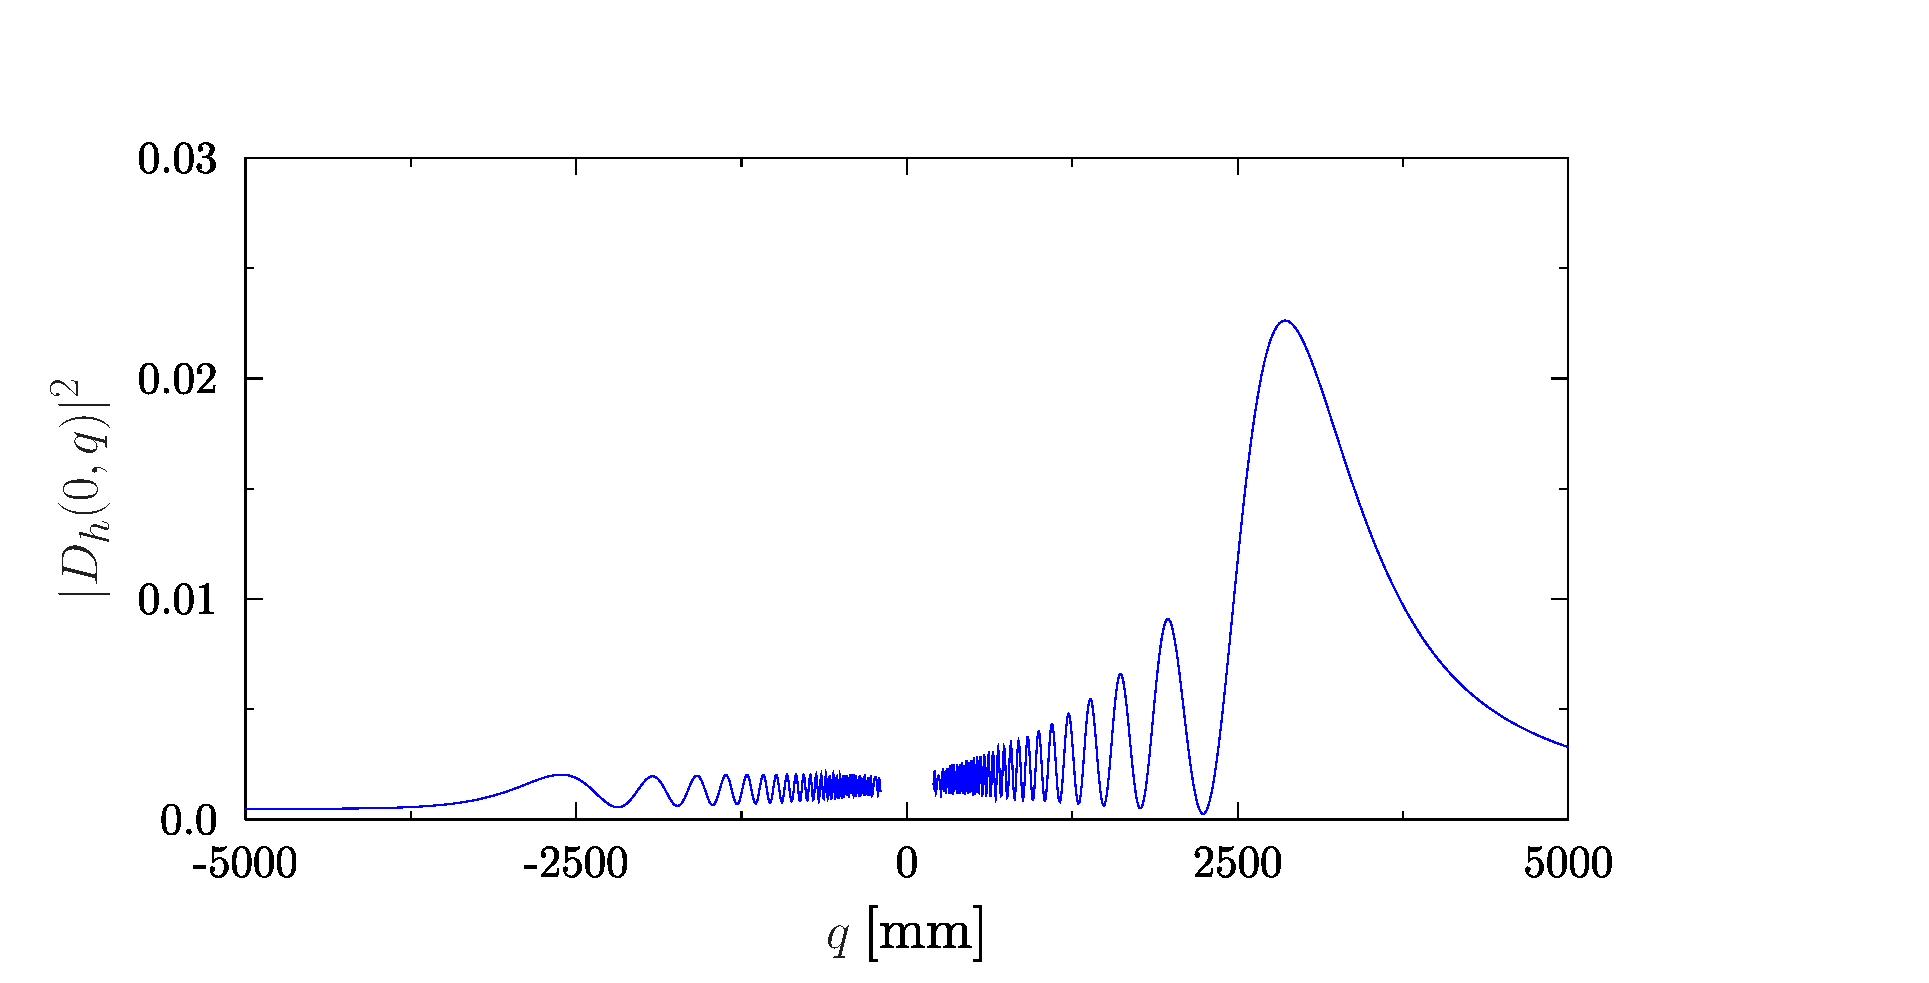
\includegraphics[width=0.95\textwidth]{flat8keV.eps}
%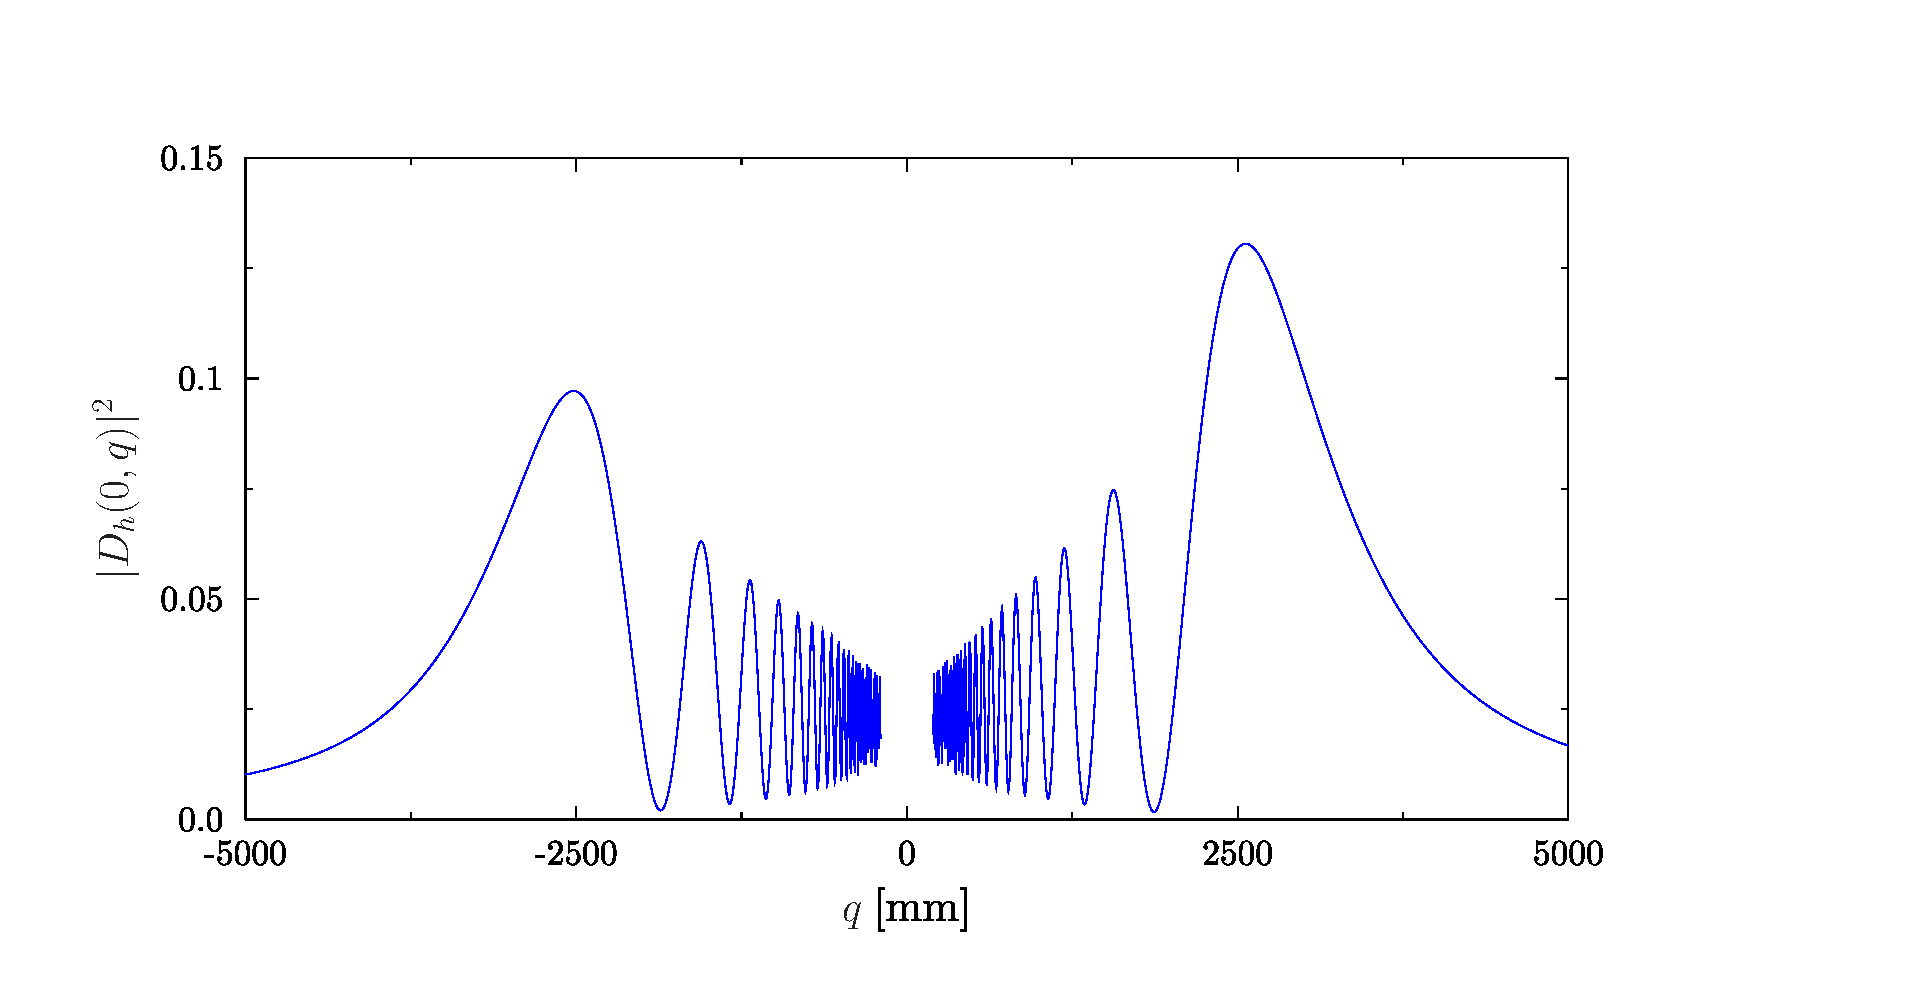
\includegraphics[width=0.95\textwidth]{flat17keV.eps}
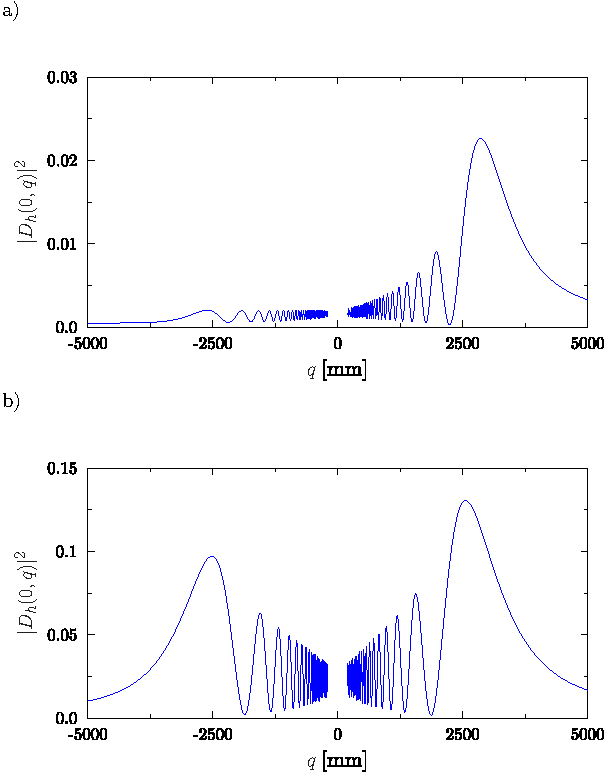
\includegraphics[width=1\textwidth]{fig4.pdf}
\end{figure}

% The moduli of the two terms in equation~(\ref{eq:approximatedDiffractedField}) are in general different: they are proportional to $\exp(\mp a \operatorname{Im}(Z))$. This is the expression of anomalous absorption (Borrmann effect). Two focusing positions are to be observed in the case of small absorption; but only one focusing position is to be observed in the case of strong absorption (see Fig.~\ref{fig:flatLaue}). It turns out that this property is also valid if the crystal plate is not flat, but cylindrically bent around an axis normal to the diffraction plane. 

% For the flat crystal under discussion, the focusing condition for a source at a finite distance $p$ from the crystal, is 
% \begin{equation}
%     \label{eq:sumpandq}
%     p+q=\pm q_{dyn}.
% \end{equation}
% This result is simply obtained by looking at the operators i) the free-space propagation from the source to the diffracting crystal, ii) effect of the crystal diffraction, and iii) the propagation downstream from the crystal to the image position. These operations  are space-invariant. They are expressed as convolutions in direct space, or simply multiplications in reciprocal space. Therefore, they can be commuted. This allows to merge the operations i) and iii) and consequently obtain equation~(\ref{eq:sumpandq}).
% Propagation through a flat crystal is space-invariant, whereas propagation through a bent crystal is not space-invariant. The reason for this difference is that, in a bent crystal case, the IF is not only dependent on the variables $(s'_0,s'_h)$, but also on the variables $(\sigma_0,\sigma_h)$, as seen in equations~(\ref{eq:TTEsimple},\ref{eq:kummer}).

\inred{
The focusing condition for a source at a finite distance $p$ from the crystal can be obtained by considering that propagation in free-space and propagation in the flat crystal are space-invariant, therefore expressed as convolutions in direct space or simple multiplications in reciprocal space. Therefore, they can be commuted. This allows to merge the free-space propagation before and after the crystal. The focusing condition is therefore
\begin{equation}
    p + q = q_{dyn}.
\end{equation}
On the contrary, propagation through a bent crystal is not space-invariant because the IF is not only dependent on the variables $(s'_0, s'_h)$, but also on the variables $(\sigma_0, \sigma_h)$ because of the factor  
$\exp[-i \vec h . \vec u (s_0, \sigma_h)]$ in 
equation~(\ref{eq:kummer}). 
}


\subsection{\inred{A new} lens equation for a bent crystal of finite thickness in symmetrical Laue geometry}
\label{sec:LaueNewCLE}

% The equations of dynamical focusing by a bent Laue crystal in symmetrical geometry used by \cite{GuigayFerrero2016} are briefly recalled in this section.

\inred{In} symmetrical Laue geometry, the factor $\exp(i \chi_0 (s'_0+s'_h))$ in equation~(\ref{eq:kummer}) is constant \inred{ on the crystal exit surface and will be omitted. Equation~(\ref{eq:kummer}) is (see Appendix~\ref{appendix:TTEintegral})}
% The equation~(\ref{eq:kummer}) can be written as
\begin{equation}
\label{eq:DhSymmetricalLaue}
    D_h(s_0,s_h) = \frac{i k}{2} \chi_h e^{-i \vec h . \vec u(s_0,\sigma_h)}
    J_0(2\sqrt{\Omega s'_0 s'_h}).
\end{equation}

% with 
% \begin{equation}
% \vec h . \vec u (s_0,\sigma_h) = \phi(\sigma_h)-\phi(s_0) =
% k \frac{\tau(\tau+a)-\xi(\xi+a)}{2 R \cos\theta_B}, 
% \end{equation}
% $s_0=(\xi+  a)/\sin2\theta_B$,
% $\sigma_h=-\tau/\sin2\theta_B$, and
% \begin{equation}
% \phi(s_0)=\frac{k \sin\theta_B}{R}(s_0^2 \sin2\theta_B - a s_0)=k \frac{\xi(a+\xi)}{2R\cos\theta_B}. 
% \end{equation}
Let us consider the incident amplitude $D_{inc}(\tau)=\exp(i k \tau^2/(2p))$, where $\tau$ is a coordinate along the axis $O\tau$ normal to $\vec k_0$ (see Fig.~\ref{fig:laue}). \inred{On the exit surface, using $s_0=(\xi+a)/\sin2\theta_B$ and $\sigma_h=-\tau/\sin2\theta_B$, and the notation $R'=R\cos\theta_B$ we obtain \inred{from equations in appendix \ref{appendix:Deformation}, in the case $\alpha=0$}

\begin{equation}
    \vec h . \vec u(s_0,\sigma_h) = k \frac{\tau(\tau+a)-\xi(\xi+a)}{ 2R'}.
\end{equation}
Using the integration variable $\eta=\xi-\tau$, the amplitude along the $\xi$-axis is, with omission of $i(k/2)\chi_h$,
}

% The diffracted wave on the axis $O\xi$
% ($q=0$) is
% \begin{equation}
%     D_h(\xi,0)=\int_{\xi-a}^{\xi+a}\frac{d\tau}{\sqrt{\lambda p}}
%     e^{ik\left[\frac{\tau^2}{2p}+\frac{\tau(\tau+a)-\xi(\xi+a)}{2R \cos\theta_B}\right]}
%     J_0(Z\sqrt{a^2-(\xi-\tau)^2}),
% \end{equation}
% or making the change of variables $\eta=\xi-\tau$,
\begin{equation}\label{eq:blabla}
    D_h(\xi,0)=\int_{-a}^{+a}\frac{d\eta}{\sqrt{\lambda p}}
    e^{\frac{ik}{2}\left[\frac{(\xi-\eta)^2}{p}+\frac{\eta^2-2\eta\xi-a\eta}{R'}\right]}
    J_0(Z\sqrt{a^2-\eta^2}).
\end{equation}
The wave amplitude at a distance $q$ downstream from the crystal is obtained using \inred{a Fresnel diffraction integral similar to} equation~(\ref{eq:Fresnel}). We thus have a double integral over $\eta$ and $\xi'$. The $\xi'$ integration \inred{is} performed analytically \cite{GuigayFerrero2013} and it turns out that
\begin{equation}
\label{eq:Dhpropagated}
    D_h(\xi,q)=
    \frac{e^{i k \frac{\xi^2}{2L}}}{\sqrt{\lambda L}}
    \int_{-a}^{+a} d\eta
    e^{\frac{ik}{2}
    [\frac{\eta^2}{L_e}-\eta(
    \frac{2\xi q_e}{q L_e}+
    \frac{a}{R'}
    )]}
    J_0(Z\sqrt{a^2-\eta^2}),
\end{equation}
where $L=p+q$, $p_e^{-1}=p^{-1}+R'^{-1}$, $q_e^{-1}=q^{-1}-R'^{-1}$ and $L_e=p_e+q_e$. The focal positions are given by $L_{e}=\pm q_{dyn}$.
% Using the notation $R'=R\cos\theta_B$, 
This can be written as
\begin{equation}
\label{eq:preLaueCLE}
    \frac{R'}{R'-q} - \frac{R'}{R' + p} = \pm \frac{q_{dyn}}{R'}.
\end{equation}
Translating equation~(\ref{eq:preLaueCLE}) in the notation of section~\ref{sec:CLE} ($p \to L_0$, $q \to -L_h$, $R \to -R_c$), we obtain
\begin{equation}
\label{eq:newCLE}
    \frac{1}{L_h-R_c \cos\theta_B} -
    \frac{1}{L_0 - R_c \cos\theta_B} =
    \pm \frac{q_{dyn}}{(R_c \cos\theta_B)^2}.
\end{equation}
If $q_{dyn}$ is set to zero, we obtain $L_h=L_0$, the same result as the lens equation~(\ref{eq:CLE}).
Equation~(\ref{eq:newCLE}) can be considered as a ``modified lens equation" which takes dynamical diffraction effects into account in symmetric Laue geometry.
We \inred{do not know an equation} like equation~(\ref{eq:newCLE}) for the general case of asymmetrical Laue diffraction. However, numerical simulations can be done to obtain the focal positions \cite{Nesterets,GuigayFerrero2016}.

Examples of numerical calculations \inred{using equation~(\ref{eq:Dhpropagated})} are shown in Fig.~\ref{fig:8keV}, for the case of the 111 reflection of a \SI{250}{\micro\meter} thick cylindrically bent symmetric Laue silicon crystal, with a curvature radius of $R$~= \SI{1}{\meter}, at a source distance $p$~= \SI{30}{\meter} and for x-ray photon energies of 8.3~keV and 17~keV. 

\inred{Alternatively, provided that the parameter $q_{dyn}$ has been previously determined numerically by a plot similar to Fig.~\ref{fig:flatLaue}, the focal positions can be given directly by equation~(\ref{eq:newCLE}). The results are in very good agreement with the focal positions obtained obtained numerically in Fig.~\ref{fig:8keV}. An important advantage in using the new CLE is that the same value of $q_{dyn}$ can be used for any value of the radius of curvature and for any value of source distance. 
}
%For both photon energy values, the effective value of $q_{dyn}$ is determined by plotting the axial intensity profile as function of $q$ for the unbent crystal of the same thickness and $p=0$ (Fig.~\ref{fig:flatLaue}). This allows to calculate $q_1$ and $q_2$ as
% \begin{subequations}
% \label{eq:q1andq2}
% \begin{align}
%     q_1 &= R' \frac{p(q_{dyn}-R')+q_{dyn}R'}{p q_{dyn}+(q_{dyn}+R')R'} \\
%     q_2 &= R' \frac{p(q_{dyn}+R')+q_{dyn}R'}{p q_{dyn}+(q_{dyn}-R')R'}.
% \end{align}
% \end{subequations}
% It can be verified that the results are in perfect agreement with the values shown by the numerical plot of the axial intensity profile. Applying the equations (\ref{eq:q1andq2})  to the cases analyzed in Fig.~\ref{fig:8keV} we get (with $q_{dyn}$=~\SI{2862}{\milli\meter} from Table~\ref{fig:flatLaue})
% $q_1$=~\SI{644}{\milli\meter},
% $q_2$=~\SI{1303}{\milli\meter}. Relative errors are -1.2\% and -2.1\%, respectively with respect to numerical values in Fig.~\ref{fig:8keV}a. For 17 keV (Fig.~\ref{fig:8keV}b)
% $q_1$=~\SI{611}{\milli\meter},
% $q_2$=~\SI{1382}{\milli\meter}, therefore the relative errors are -2.24\% and 0.7\%, respectively.
% In these cases,
% $\operatorname{Im}(Za)$ is negative. It means that the focus position with lowest absorption (therefore with largest intensity) is $q_1$. This is in agreement with the numerical plots. 
% The highest peak is for $q_1<q_2$ at the x-ray energy of 17 keV. At the energy of 8 keV, only the  peak $q_1$ is present and the $q_2$ peak is damped out because the anomalous absorption effect.

We are often interested in real focusing ($q>0$) of an incident beam from a very distant real source, for instance in dispersive EXAFS beamlines. 
% $q_1$ and $q_2$ are both decreasing functions of $p$. 
Suppose $0<R'\le q_{dyn}$. When $p$ increases from zero to infinity, $q_1$ decreases from $q_1=R'q_{dyn}/(q_{dyn}+R')$ to 
% $q_1=R'(1-R'/q_{dyn})$.
$q_1=R' q_{dyn}(q_{dyn}-R')$.
Simultaneously, $q_2$ decreases from $q_2=R'q_{dyn}/(q_{dyn}-R')$ to 
% $q_2=R'(1+R'/q_{dyn})$.
$q_2=R'q_{dyn}(q_{dyn}+R')$.
For very large $p$-values, we have the simple relation $q_1+q_2\approx 2R'$ \inred{in good agreement with the numerical results in Fig.~\ref{fig:8keV}.}

\begin{figure}
\label{fig:8keV}
\caption{Numerical evaluation of diffracted intensity by a \SI{250}{\micro\meter} thick Si 111 symmetric Laue crystal calculated using equation~(\ref{eq:Dhpropagated}) for a bent (R~= \SI{1}{\meter}) crystal and $p$~= \SI{50}{\meter}. 
a) on-axis intensity for a photon energy of 8.3 keV. 
Inset: transverse profile at the focal distances (maximum values):  
$q_1$~= \SI{651}{\milli\meter} (blue), and
$q_2$~= \SI{1330}{\milli\meter} (red).
b) on-axis intensity for a photon energy of 17 keV.
Inset: transverse profile at the focal distances (maximum values):
$q_1$~= \SI{625}{\milli\meter} (blue), and 
$q_2$~= \SI{1372}{\milli\meter} (red).
}
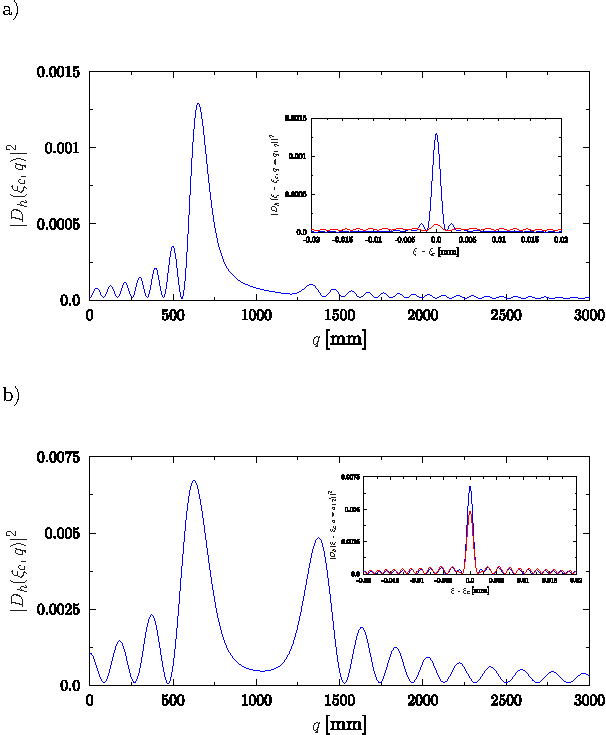
\includegraphics[width=1\textwidth]{fig5.pdf}

% 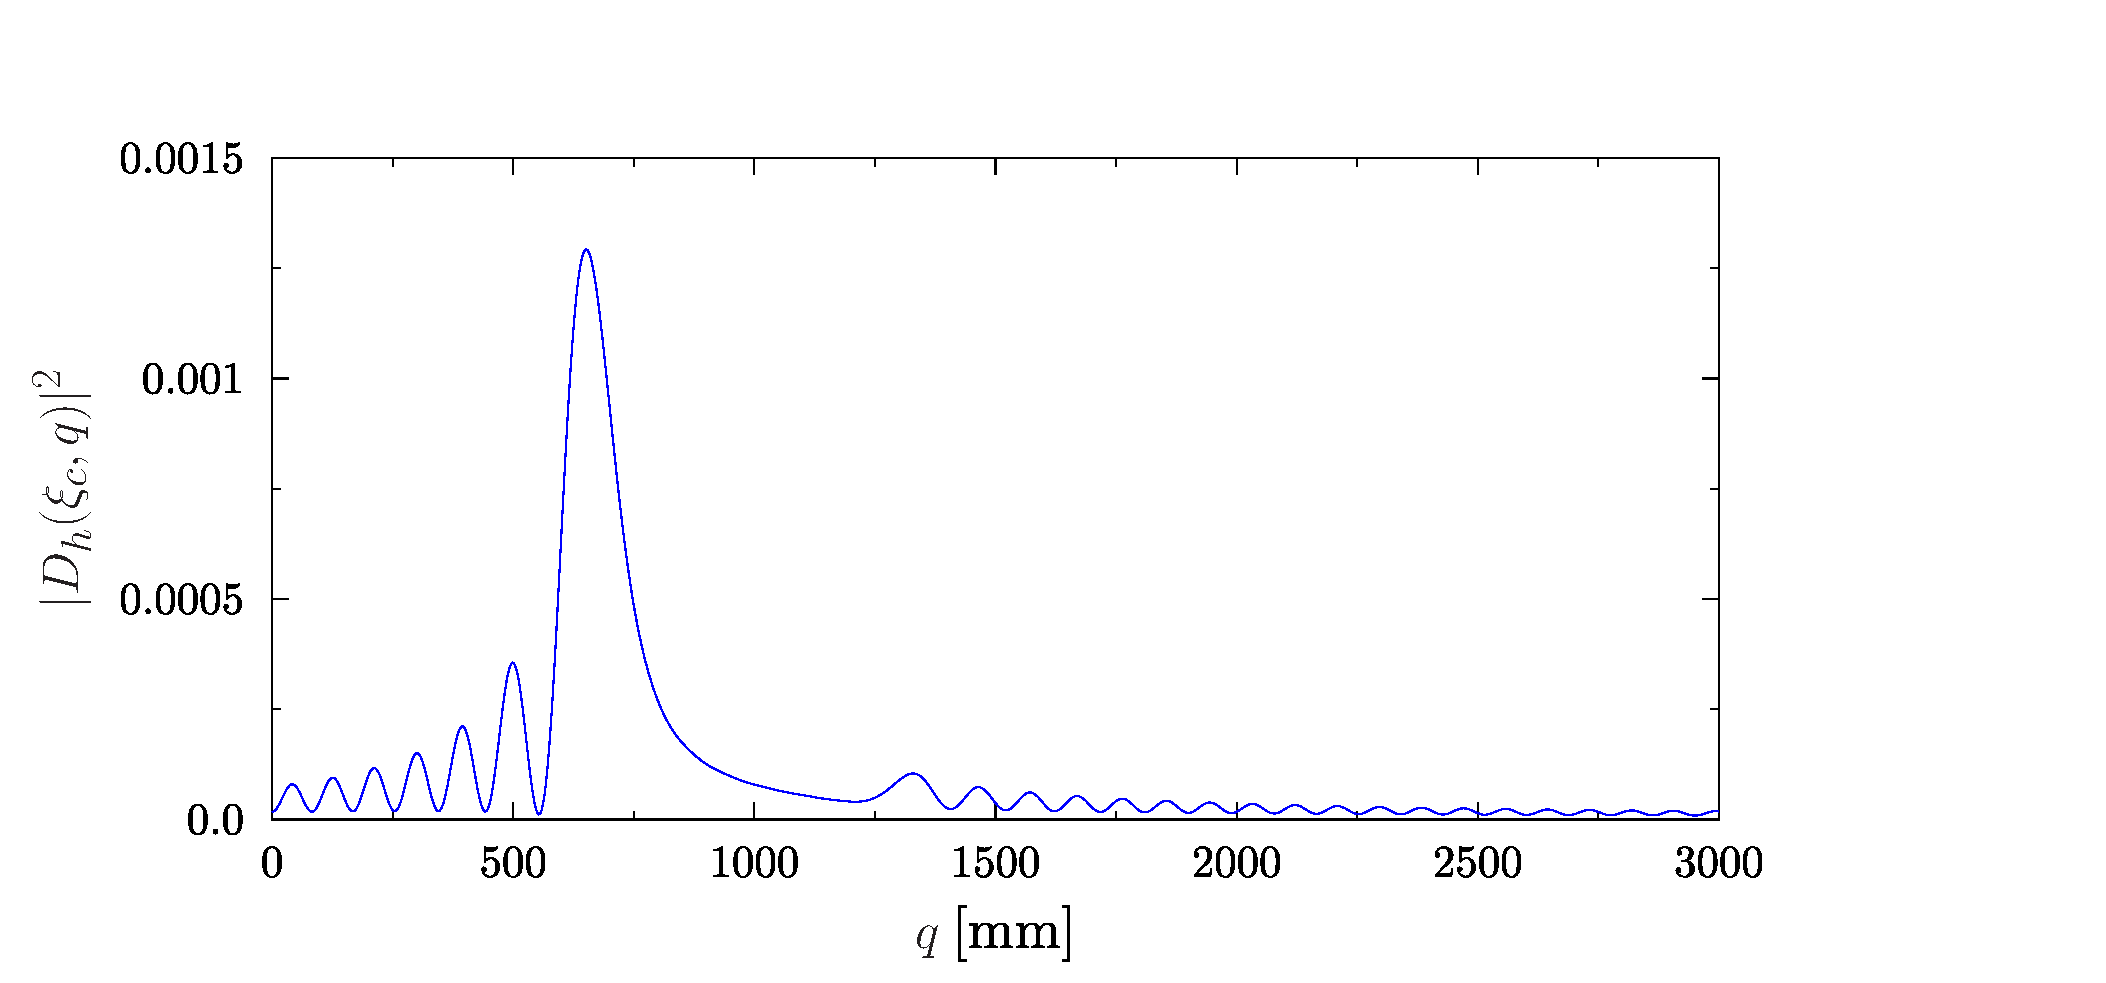
\includegraphics[width=0.96\textwidth]{bent1m8keV.eps}

% \begin{picture}(0,0)
% \setlength{\unitlength}{1cm}
% \put(-1.5,3){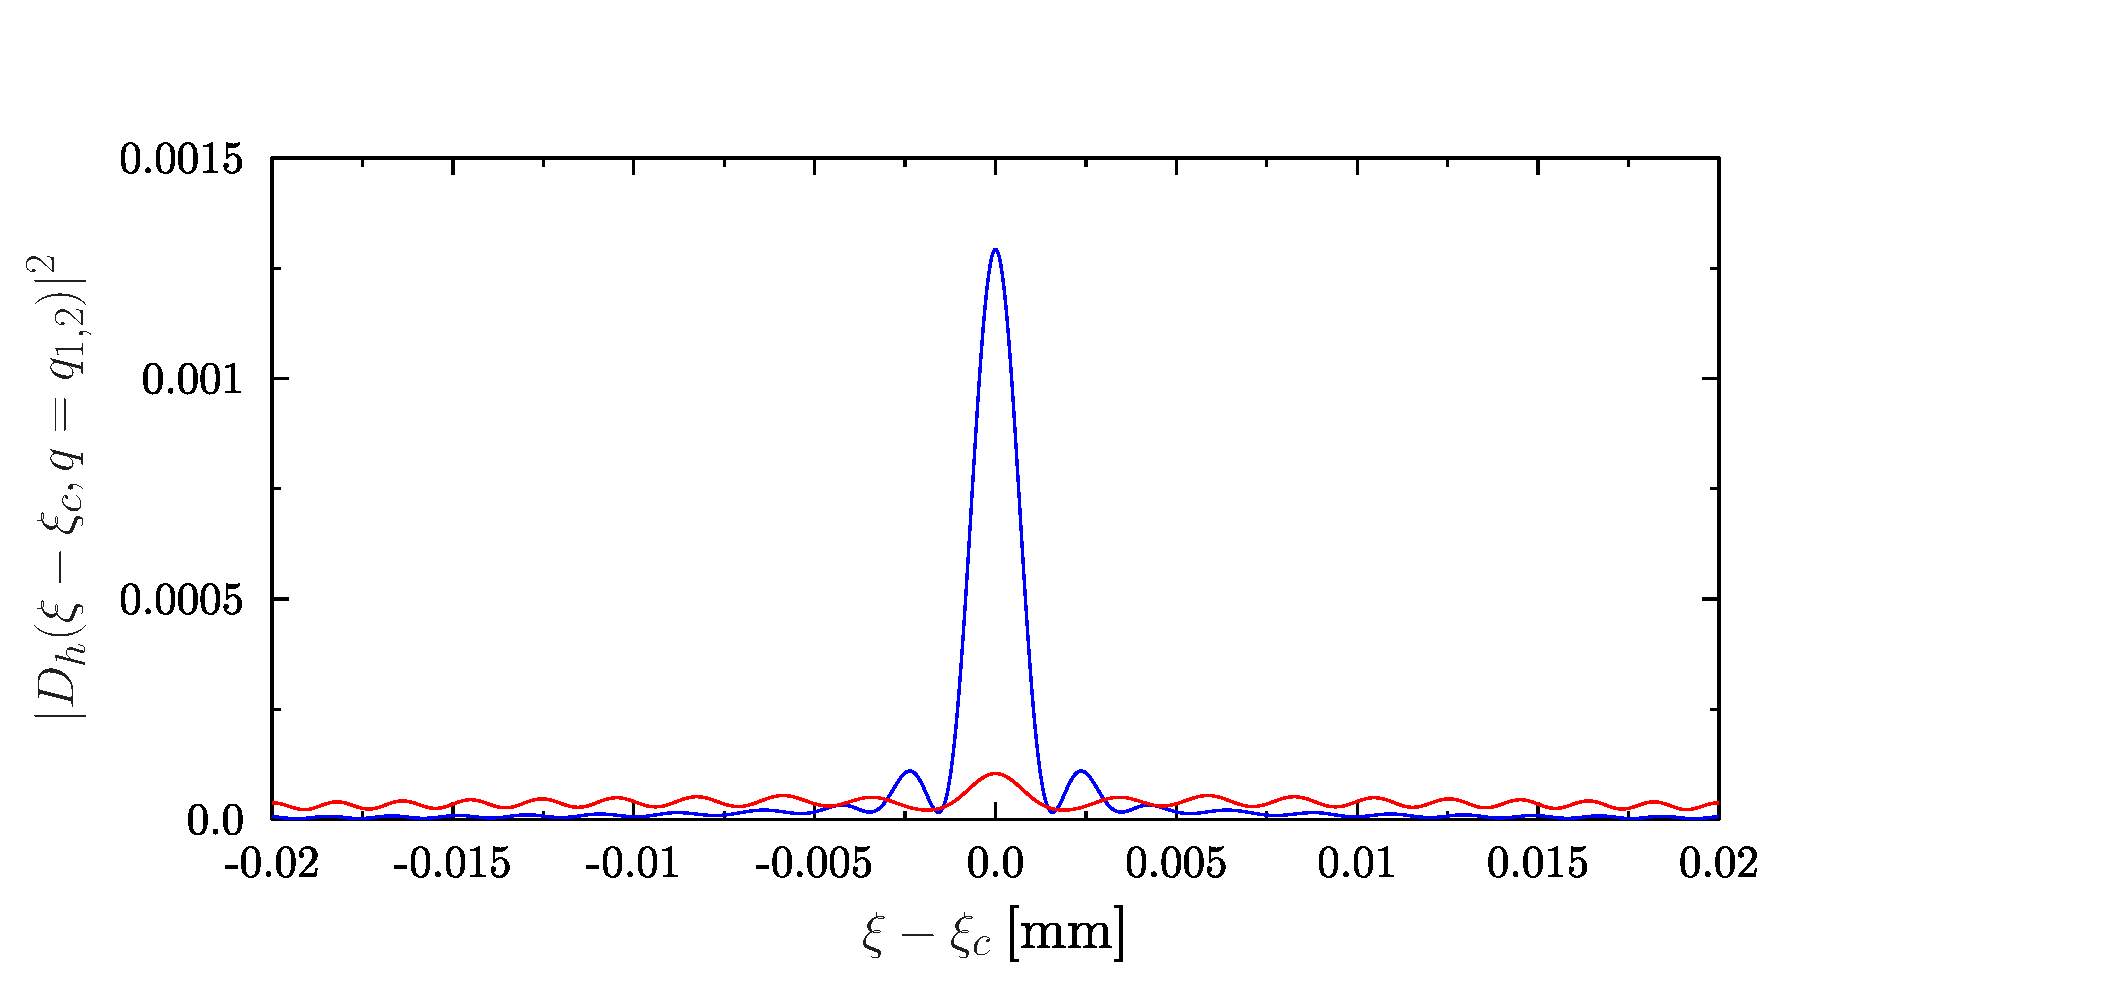
\includegraphics[width=0.46\textwidth]{bent1m8keV_profile.eps}}
% \end{picture}

% 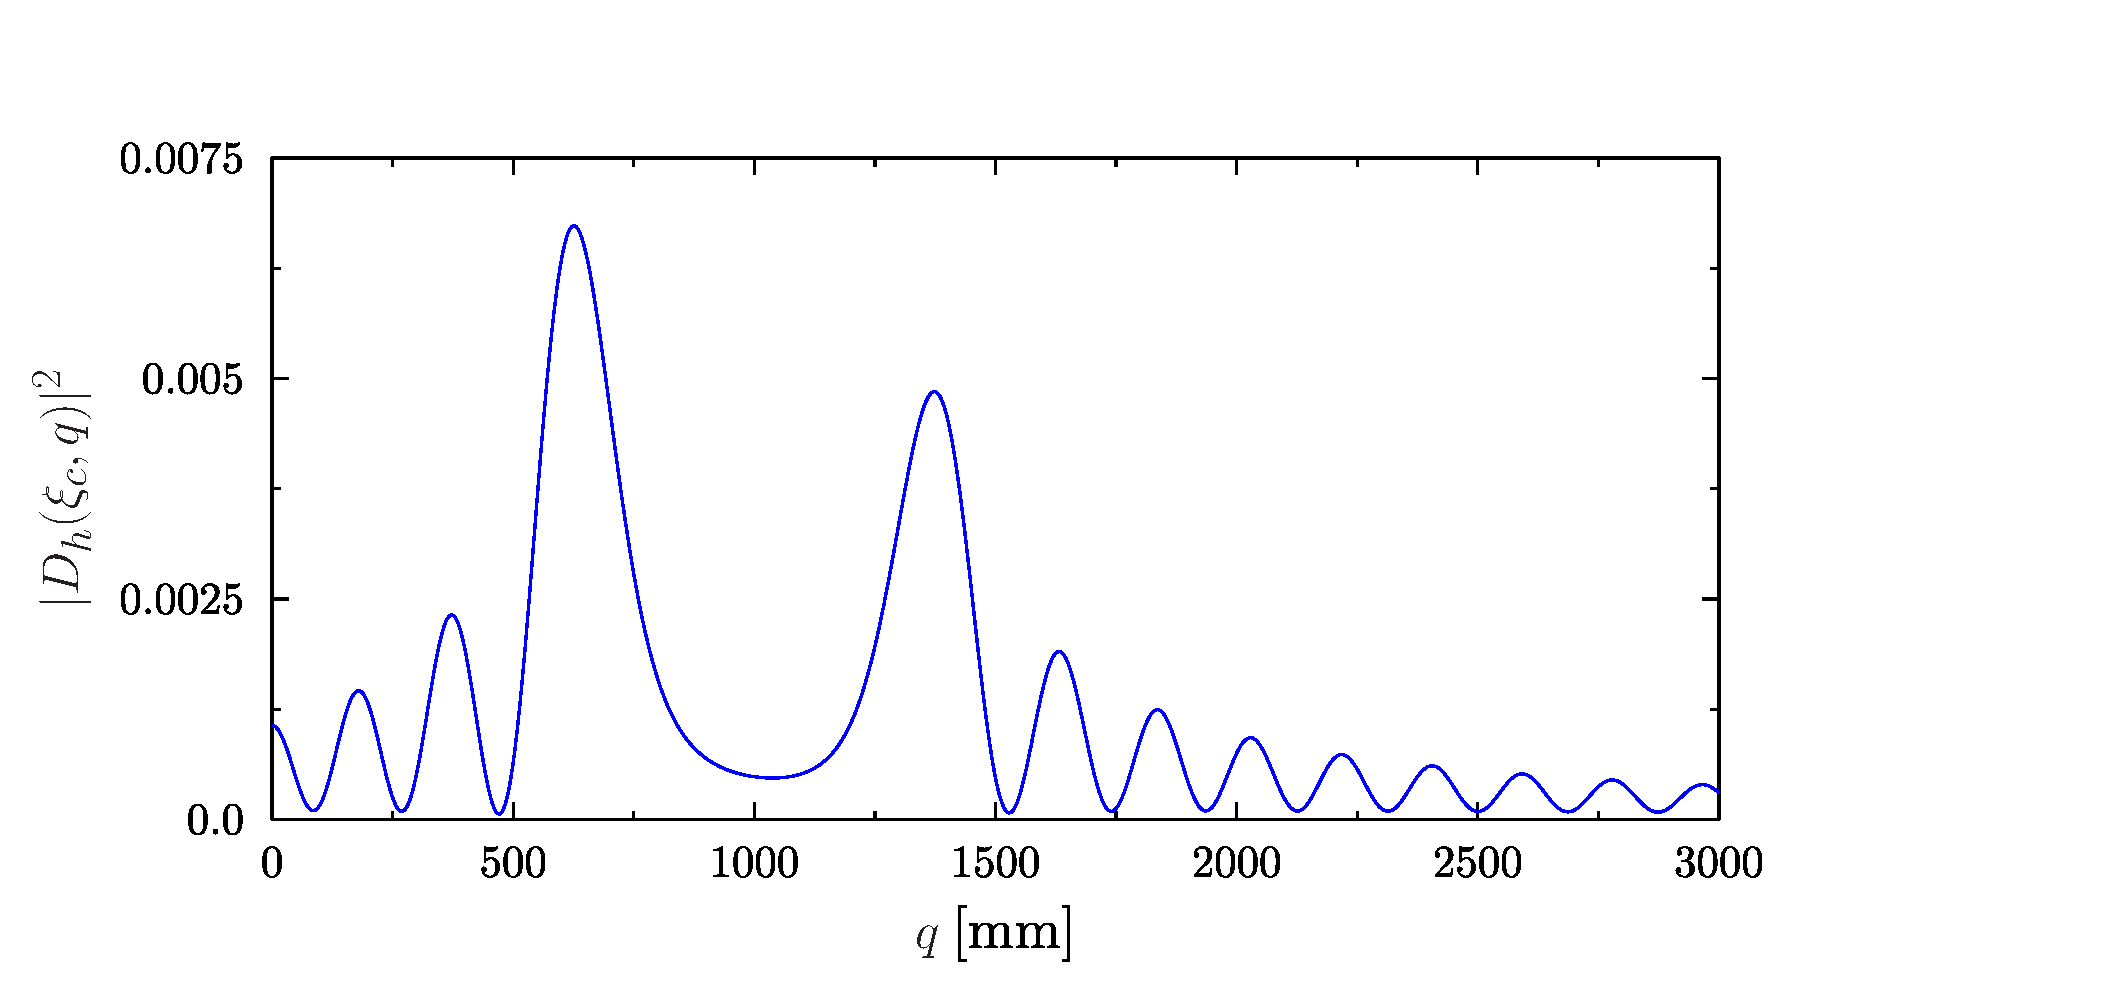
\includegraphics[width=0.96\textwidth]{bent1m17keV.eps}

% \begin{picture}(0,0)
% \setlength{\unitlength}{1cm}
% \put(-1.1,3){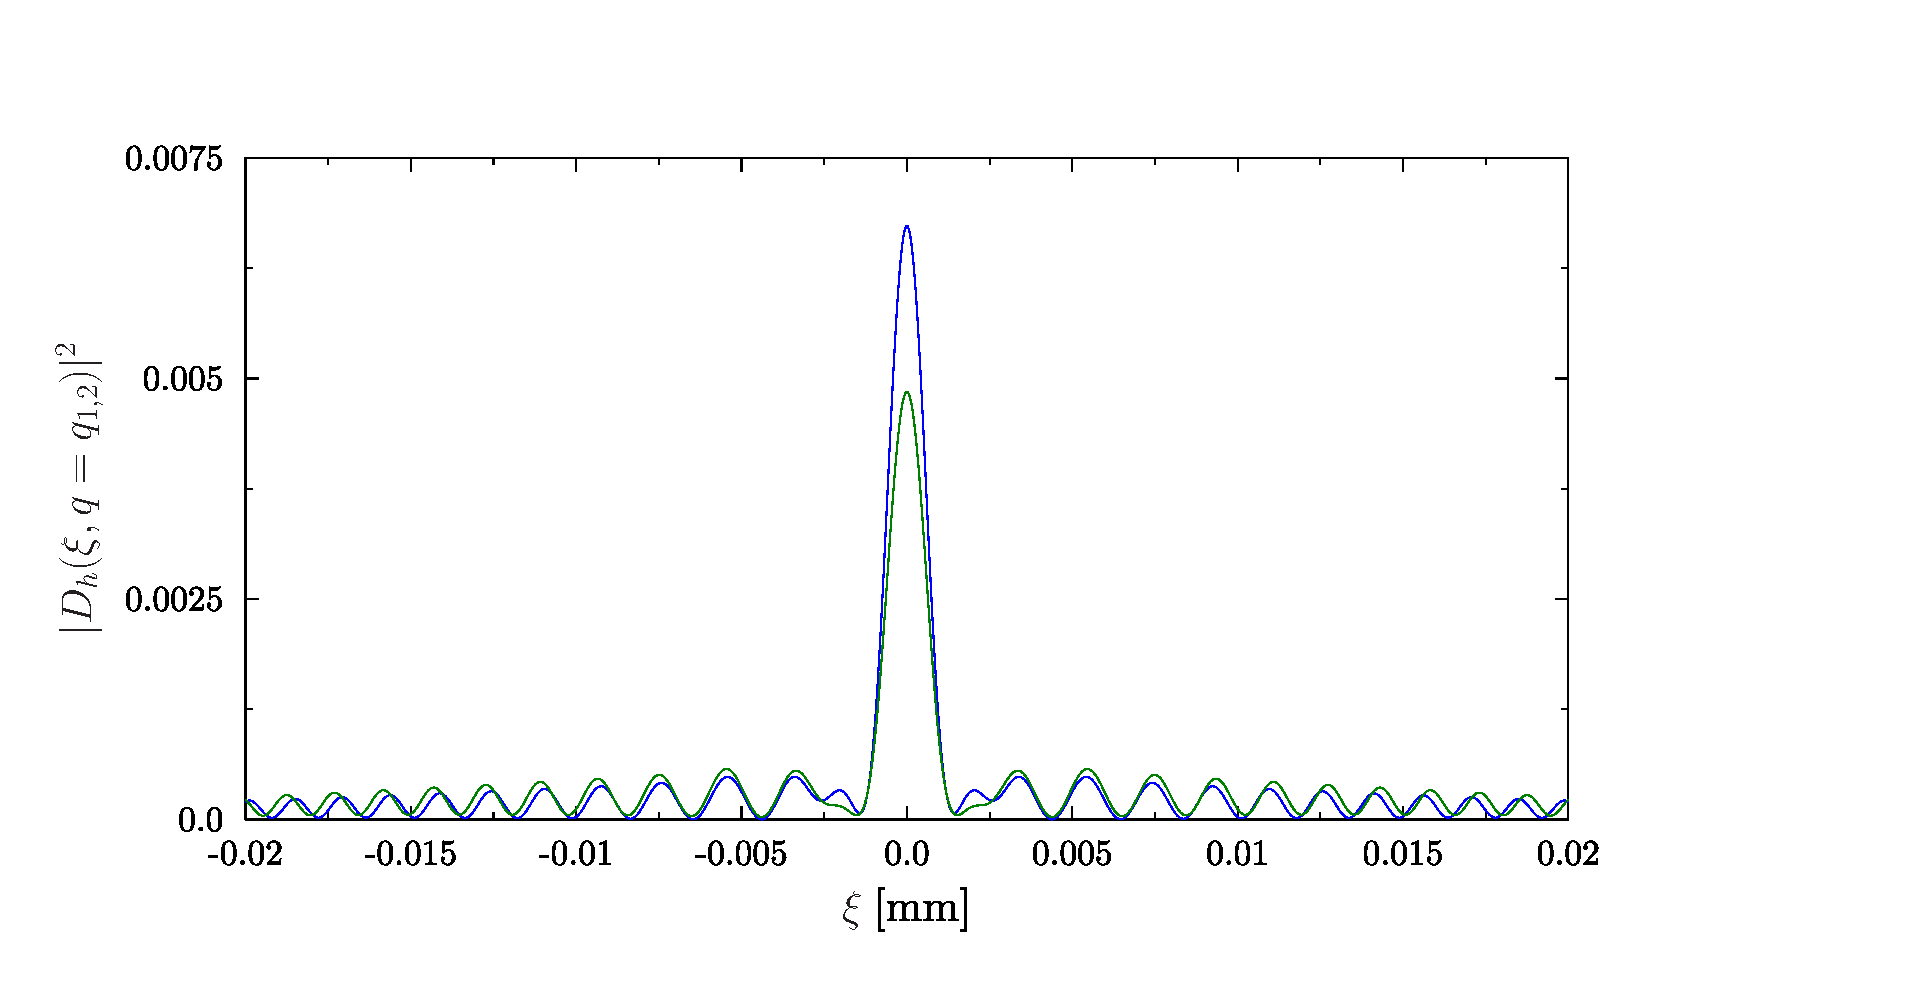
\includegraphics[width=0.46\textwidth]{bent1m17keV_profile.eps}}
% \end{picture}

\end{figure}

It can be seen from equation~(\ref{eq:Dhpropagated}) that the intensity function $|D_h(s_0,s_h)|^2$ as a function of $\xi$ is symmetric around $\xi_c=-a q L_e / (2 q_e R')$. This denotes a lateral shift of the intensity profile \inred{from its position for the unbent crystal} (the axial intensity profiles of Fig.\ref{fig:8keV}a and \ref{fig:8keV}b are actually \inred{plotted} as a function of $(\xi-\xi_c))$.
%\todo{ Discuss how it changes... Make a plot vs $\xi$: IT CHANGES  $\approx -a/2$... TOO MUCH??}

\subsection{Semianalytical approach in asymmetric Laue geometry \inred{and its CLE limit}}
\label{sec:LaueCompatibilityCLE}

% % In this section we demonstrate, for the general case of asymmetric Laue, how the CLE can be obtained from the dynamical theory in the limit of zero thickness. 

% \inred{Here we follow the analytic process used in the preceding section to obtain equation~(\ref{eq:blabla}). The formulation is however more complicated, because of the much larger number of involved parameters and the mathematical complexity of the Kummer function. 
% }
% % To obtain this result we first summarize the results of \cite{GuigayFerrero2016} that give the expression of the diffracted field at the exit face of the crystal, which is then propagated to the image at a distance $q$. This expression has to be evaluated numerically (semi-analytically). It is shown that in the limit of zero thickness, this expression corresponds to a cylindrical wave focused in a position dictated by an expression that coincides with the CLE.
% % The same procedure used in section~\ref{sec:LaueNewCLE} is applied here, but it is more complicated for asymmetric reflection because of the larger number of parameters and the mathematical complexity of the Kummer function. 
% The reflected amplitude versus the $\xi$ coordinate at negligible distance from the exit crystal surface is expressed by the following integral over the variable $\eta=\xi-\tau/\gamma$
 \inred{The generalizartion of equation (\ref{eq:blabla}) to asymmetric Laue geometry is \cite{GuigayFerrero2016}}
\begin{equation}
\label{eq:unpropagatedkummer}
    D_h(\xi,0) = 
    \int_{-a}^{a} \gamma\frac{d\eta}{\sqrt{\lambda p}}
    e^{i k \gamma^2
    \frac{(\xi-\eta)^2}{2p}+i \phi(\xi,\eta)
    }
     M(\frac{i\Omega}{A},1,i g k \frac{a^2-\eta^2}{R}),
\end{equation}
where 
%$\gamma=\cos\theta_1/\cos\theta_2$, $a=t \sin\theta_B/(2\cos\theta_1)$,
\begin{multline}
    \phi(\xi,\eta) =\frac{k}{2R}[-\mu_2\gamma^2(\xi-\eta)^2
    +a_2\gamma(\eta-\xi) \\
    -\mu_1(a+\xi)^2 
    +a_1(a+\xi)
    -2g(a+\xi)(\xi-\eta)].
\end{multline}
The parameters $\mu_{1,2}$, $a_{1,2}$ \inred{and $g$} are given in Appendix~\ref{appendix:Deformation},
% $g=A\gamma R/ k \sin^22\theta_B$,
% and $\rho=\nu/(1-\nu)$ with $\nu$ the Poisson ratio.   
The reflected amplitude $D_h(\xi,q)$ at distance $q$ downstream \inred{from} the crystal is again obtained \inred{as in} equation~(\ref{eq:Fresnel}), therefore by double integration over $\eta$ and $\xi'$. The $\xi'$-integration can be again performed analytically. The remaining $\eta$-integration involving the Kummer function is carried out numerically \cite{GuigayFerrero2016}. We consider this approach as semi-analytical, in contrast to the approach used by \cite{Nesterets} which is based on a numerical solution of the TTE.

\inred{It is interesting to study analytically the limit of this semi-analytical formulation in the case of}
% We are now interested in the limit this semi-analytical formulation in the case of 
vanishing crystal thickness ($a\rightarrow0{}$) \inred{because the comparison with lens equation~(\ref{eq:CLE}) represents a validity test of the semi-analytical formulation. 
In the limit ($a\rightarrow0{}$),}
the Kummer function is equal to unity in equation~(\ref{eq:unpropagatedkummer}), and the integral can be replaced by $2a$ times the integrand evaluated at $\eta=a=0$, therefore


\begin{equation}
\label{eq:14reduced}
    D_h(\xi,0) = \frac{2 a \gamma}{\sqrt{\lambda p}} e^{\frac{i k \xi^2}{2}(\frac{\gamma^2}{p}-\frac{\mu_2\gamma^2+\mu_1+2g}{R})}.
\end{equation}

This is the expression of the amplitude of a cylindrical wave focused at the distance $q$ such that
\begin{equation}
    \frac{1}{q}+\frac{\gamma^2}{p}-\frac{\mu_2\gamma^2+\mu_1+2g}{R}=0. 
\end{equation}
Using the identity
\begin{equation}
\label{eq:appendixIdentity}
    \mu_1+\gamma^2\mu_2+2g=\frac{\cos\theta_2-\cos\theta_1}{\cos^2\theta_2},
\end{equation}
which is \inred{derived} in Appendix~\ref{appendix:Deformation}, the focusing condition is 
\begin{equation}
    \frac{1}{q}+\frac{\gamma^2}{p}+\frac{\cos\theta_1-\cos\theta_2}{R\cos^2\theta_2}=0,
\end{equation}
or,
\begin{equation}
    \frac{\cos^2\theta_2}{q}+\frac{\cos^2\theta_1}{p}+\frac{\cos\theta_1-\cos\theta_2}{R}=0,
\end{equation}
which is the CLE (equation~(\ref{eq:CLE})) for the Laue case, with the correspondence $p \rightarrow L_0$, $q \rightarrow -L_h$, $R \rightarrow -R_c$, $\theta_1 \rightarrow \varphi_0$ and $\theta_2 \rightarrow \varphi_h$


\section{Polychromatic geometric focusing}
\label{sec:polychromatic}
%
% Dear Dr. Guigay,
% Good morning.
% I read your recent preprint on arXiv with great interest (X-ray focusing
% by bent crystals: focal positions as predicted by the crystal lens
% equation and the dynamical diffraction theory ). There is a citation to
% my work in 2019 (Focusing and energy dispersion properties of a
% cylindrically bent asymmetric Laue crystal). Thank you for citing it.
% I noticed the note to that citation "(Qi et al., 2019) FOUND another
% polychromatic condition in Laue geometry. A single-ray focusing … ",
% and I need to clarify that the 'single-ray focusing' is not found by our
% work. Our work (Qi et al., 2019) explained it with more details and made
% development on top of it, but the 'single-ray focus' was first studied
% by Suortti 1994, 1997 at ESRF (attached to the email) and they were
% cited in our paper.
% I want to clarify this in case of confusion by the word 'found'.
% I admire your works and I have learned a lot by reading many of your
% publications as we have common research interests in crystal optics.
% Thank you very much.
% By the way, we recently had a publication on the _Journal of Applied
% Crystallography_
% (https://scripts.iucr.org/cgi-bin/paper?S1600576720016428) that
% interpreted bent Laue optics in a new approach and found a different
% type of monochromatic focusing for 'thick crystals'. Some preliminary
% experiment has shown evidence to this theoretical finding. I have
% attached a copy to this email and hope it will be of your interest too.
% Best regards,
% Peng Qi
% PostDoc - Department of Anatomy, Physiology, and Pharmacology 

As pointed out by \cite{CK}, the monochromatic focusing \inred{condition} must not be confused with the polychromatic focusing \inred{condition} \cite{handbook,Caciuffo1987,Schulze1998,Martinson}, obtained by varying the wavelength of the reflected rays in order to satisfy the exact Bragg condition on the \inred{whole} crystal surface.
% (the position of the point $O$ and the change of the Bragg angle along the crystal surface. 
% The asymmetry angle $\alpha$ is constant. 
The equation $\varphi_0+\varphi_h=2\alpha$ in Laue case\inred{, or $\varphi_0+\varphi_h=2\alpha+\pi$ in Bragg case,} implies $\Delta\varphi_0+\Delta\varphi_h=0$. Using equations~(\ref{eq:angles}) and  (\ref{eq:angles2}) we obtain
\begin{equation}
\label{eq:polychromaticfocusing}
\frac{{\cos {\varphi _o}}}{{{L_0}}} + \frac{{\left| {\cos {\varphi _h}} \right|}}{{{L_h}}} = \frac{2}{R_c}.
\end{equation}
% or, in the notation of section~\ref{sec:dynamlicalLaue}, $-\cos\theta_1/p + |\cos\theta_2|/q=2/R$.
Equation~(\ref{eq:polychromaticfocusing}) is usually referred to as the "geometric focusing" condition for bent crystals. It is also applied in the case of flat crystals \cite{sanchezdelrio1994}. \inred{Like in equation~(\ref{eq:CLE}), the crystal thickness does not appear in equation~(\ref{eq:polychromaticfocusing}).}
\inred{The combination of equations (\ref{eq:CLE}) and (\ref{eq:polychromaticfocusing}) gives

\begin{equation}
\label{eq:coincidence}
\frac{\cos\varphi_0}{L_0}(\cos\varphi_h+\cos\varphi_0) = \frac{|\cos\varphi_h|}{L_h}(\cos\varphi_h+\cos\varphi_0),
\end{equation}
which is verified either in the symmetric Bragg case ($\cos\varphi_h+\cos\varphi_0=0$), or if $\cos\varphi_0/L_0=|\cos\varphi_h|/L_h=1/R$, which is the Rowland condition. The Rowland condition is therefore necessary for the coincidence of equations (\ref{eq:CLE}) and (\ref{eq:polychromaticfocusing}) in Laue geometry.
\footnote{This is different from the statement of \cite{CK} that the coincidence is always realised under symmetrical reflection or the Rowland condition.}
}




% coincide in the symmetric Bragg case for which $\cos\varphi_o=-\cos\varphi_h=\sin\theta_B$. 
% In the symmetric Laue case, for which $\cos\varphi_o=\cos\varphi_h=\cos\theta_B$,  condition (\ref{eq:CLE}) is reduced to $L_0=L_h$ and equation~(\ref{eq:polychromaticfocusing}) is then $L_0=L_h=R_c\cos\theta_B$, which corresponds to Rowland geometry. Therefore \inred{conditions} (\ref{eq:CLE}) and (\ref{eq:polychromaticfocusing}) coincide \inred{in} symmetric Laue case only if the Rowland condition is satisfied.\footnote{\cite{CK} stated that they coincide if a symmetrical reflection is used {\it or} the Rowland condition is fulfilled, which is false in the symmetric Laue off-Rowland}

% The conditions (\ref{eq:CLE}) and (\ref{eq:polychromaticfocusing}) \inred{always} coincide \inred{in} the Rowland condition $L_0=R_c\cos\varphi_0$, as they both give $L_h=R_c|\cos\varphi_h|$. 
A narrow energy band \inred{is reflected in Rowland condition}, because the angle of incidence on the local reflecting plane does not change along the bent crystal surface.
\inred{
On synchrotron dispersive EXAFS beamlines, the use of a Bragg symmetric reflection by a bent polychromator at a large distance from the source guarantees the focusing of a broad bandwidth (up to $~1$ keV) on a small spot \cite{Tolentino:ms0206} at a distance close to $L_h=(R_c\sin\theta_B)/2$. 
}
Laue polychromators are also used in synchrotron beamlines.
% As discussed \inred{above}, \inred{the coincidence of
% conditions (\ref{eq:CLE}) and (\ref{eq:polychromaticfocusing}) is impossible in off-Rowland configuration, which would provide} a large energy bandwidth. 
% However, 
\inred{In symmetric Laue geometry, condition (\ref{eq:CLE}) should be replaced by equation~(\ref{eq:newCLE}), which is $L_h \approx R_c \cos\theta_B + (R_c \cos\theta_B) ^2 / q_{dyn}$ if the source distance is very large.} 
\inred{Coincidence with (\ref{eq:polychromaticfocusing}) is then obtained} if
% $R_c \cos\theta_B /2 = R_c \cos\theta_B+ (R_c \cos\theta_B) ^2 / q_{dyn}$ which implies 
$R_c=-q_{dyn}/(2\cos\theta_B)$,
\inred{which means} real focusing at the distance $|L_h|=q_{dyn}/4$ with beam incidence in the \inted{crystal} convex side ($R_c<0$). 
\inred{If $|L_h|$ is fixed, the required conditions are $|R_c| = 2 |L_h| / \cos\theta_B$ and $q_{dyn}=4|L_h|$. The last condition should be fulfilled by choosing} the crystal thickness, as in  \cite{Mocella2004,Mocella2008}.

\inred{Another polychromatic condition for Laue geometry has been introduced more recently \cite{Martinson, PengQi, PengQi2021}.
The energy components of a polychromatic ray traversing a bent Laue crystal with finite thickness meet the Bragg condition at different positions along the ray path. They are diffracted with different Bragg angles, therefore they exit in different directions, giving raise to a polychromatic focus from a single ray. The ``magic contition", under which single ray focusing and geometric focusing (equation (\ref{eq:polychromaticfocusing})) would coincide, is achieved by the adequate choice of the asymmetry. The magic condition is independent of the crystal thickness \cite{PengQi2021}. We observe that the magic condition (equation (19) in \cite{PengQi2021}) and the modified lens equation (\ref{eq:newCLE}) are both satisfied in the particular case of symmetric Laue geometry in Rowland configuration.   

}

\section{Conclusions \inred{and future perspectives}}
\label{sec:summary}


\inred{The} crystal lens equation (CLE, equation~(\ref{eq:CLE})) based on the conservation of the parallel component of the wavevector in the diffraction process \inred{has been revisited}. It includes all cases of symmetric and asymmetric Laue and Bragg geometries. It differs from the previous formulation \cite{CK} in the Laue case. However, \inred{in Laue geometry,} the lens equation 
% is actually of little practical interest in the Laue case, because it 
can be only applied if the crystal is \inred{so thin that} important effects resulting from the dynamical theory of diffraction, like the focusing of the Borrmann triangle, \inred{can be neglected}. We derived the modified lens equation (\ref{eq:newCLE}) which overcomes this restriction \inred{in the Laue symmetric case}. Consistently, it converges to the CLE if the crystal thickness \inred{tends to zero}. The generic case of arbitrary asymmetry is left for a future investigation.
\inred{The fact that dynamic focusing cannot be achieved in Bragg case (see Appendix D) justifies in some way the larger applicability of the CLE in Bragg case. }


The application of the CLE (equation~\ref{eq:CLE}) is restricted to monochromatic focusing. Polychromatic focusing, as used in the polychromators of dispersive EXAFS beamlines, happens when the wavelength of the reflected rays changes to exactly match the Bragg angle. This condition is given by a different lens equation (\ref{eq:polychromaticfocusing}). This implies a specular reflection of the rays on the Bragg planes that is, in general, incompatible with the CLE or the results of dynamical theory, except for the Bragg symmetric case. It has been demonstrated that focii predicted by monochromatic and polychromatic focusing conditions coincide if the source is situated on the Rowland circle. Moreover, such coincidence is also true for any source position (off-Rowland) in symmetric Bragg geometry, but not in symmetric Laue geometry. Here, for the Laue symmetric case, both polychromatic and monochromatic focii can match if the modified lens equation~(\ref{eq:newCLE}) is used instead, but requires a particular choice of the crystal thickness.
\inred{The additional effect of focusing a polychromatic ray \cite{PengQi2021} gives the ``magic condition"  for Laue focusing, which implies geometric and single scattering. Further studies would be required to match the magic condition (which does not depend on the crystal thickness) with monochromatic focusing. This could be done by optimizing numerically the crystal thickness using the formulation in section~\ref{sec:LaueCompatibilityCLE}. }

% The case of symmetric Bragg geometry seems to be of particular practical interest, because of simultaneous polychromatic and monochromatic focusing. Moreover, the CLE can then be used to predict the focus position with good accuracy. Therefore, the CLE appears to be more relevant in the Bragg case rather than in the Laue case.


% \ack{Acknowledgements}
% A large part of this work comes from ...


\bibliography{iucr} % reads iucr.bib with items
\bibliographystyle{iucr}
%\referencelist{library}

\appendix
\section{\inred{Derivation of the} Lens Equation from the phase-factor of the Takagi-Taupin equations}
\label{appendix:CLE}

\inred{Under} a deformation field $\vec u(\vec r)$, the crystal polarizability \inred{is} taken as 
$\chi(\vec r-\vec u(\vec r))$, where $\chi(\vec r)$ is the
polarizability of the non-deformed crystal. The Fourier components of the electric susceptibility $\chi_{h,\bar h}$ are multiplied by the phase factors $\exp(-  \vec h . \vec u (\vec r))$ and $\exp(\mp i \vec h . \vec u (\vec r))$, respectively, in the TTE.
In the case of a very thin crystal, the ray \inred{reflected at position} $x$ on the \inred{bent} crystal surface is simply affected by the phase factor 
\begin{equation}
    \label{eq:phasefactor11}
    e^{-i \vec h . \vec u(x)} = e^{i k (\cos\varphi_h-\cos\varphi_0) \frac{x^2}{2 R_c} },
\end{equation}
which is obtained using $\vec u(x) = -(x^2/(2R_c))\vec n$ and $\vec n . \vec h = \vec n.(\vec k_h - \vec k_0) = k(\cos\varphi_h-\cos\varphi_0)$. 

\inred{In the case of the undeformed crystal, the incident \inred{amplitude} $\exp[i k \tau^2 / (2L_0)]$, \inred{along the axis} $O\tau$ 
% perpendicular to the direction $Os_0$ of Bragg incidence (see Fig.~\ref{fig:laue}), 
is translated into 
\begin{equation}
    D_{inc}(\xi) = e^{i k \frac{\xi^2}{2L_0}\left(\frac{\cos\varphi_0}{\cos\varphi_h}\right)^2},
\end{equation}
% $\exp[i k \xi^2\gamma^2 / (2L_0)]$ 
along the axis $O'\xi$ (see Fig.~\ref{fig:laue}).
This is combined with equation (\ref{eq:phasefactor11}) to obtain} the amplitude of the Bragg-reflected wave along the axis $O\xi$
\begin{equation}
\label{eq:A4}
    D_h(\xi) = e^{i k
    \frac{\xi^2}{\cos^2\varphi_h}\left(\frac{\cos\varphi_h-\cos\varphi_0}{2R_c} + \frac{\cos^2\varphi_0}{2L_0}\right)},
\end{equation}
corresponding to a real or virtual focus if the phase of this function is negative or positive respectively. 

\inred{Using the convention defined in section~\ref{sec:CLE} (see Fig.~\ref{fig:geometries}), a real focus requires $L_h<0$ in Laue case and $L_h>0$ in Bragg. A cylindrical converging wave has then the form $\exp(i k \xi^2 / (2L_h))$ in Laue and $\exp(-i k \xi^2 / (2L_h))$ in Bragg (we arrive to the same result considering a virtual focus). For both Bragg and Laue cases we can write}

\begin{equation}
\label{eq:A5}
D_h(\xi) = e^{i k \frac{\xi^2}{2 L_h}\frac{|\cos\varphi_h|}{\cos\varphi_h}}.   
\end{equation}
 Comparing equations~(\ref{eq:A4}) and (\ref{eq:A5}), we finally obtain
\begin{equation}
    \frac{\cos\varphi_h-\cos\varphi_0}{R_c}+
    \frac{\cos^2\varphi_0}{L_0}=\frac{|\cos\varphi_h|\cos\varphi_h}{L_h},
\end{equation}
which is equivalent to the lens equation (\ref{eq:CLE}).

\section{Derivation of the influence functions \inred{equation (\ref{eq:kummer})} from the integral form of the Takagi-Taupin equations}
\label{appendix:TTEintegral}

\inred{For a point source in position $(\sigma_0,\sigma_h)$ on the crystal surface, the incident amplitude has the form $D_{inc}= \delta(s_h-\sigma_h)$.}
% , corresponding to $D_{inc}=\delta(s_h-\sigma_h)$.
The refracted amplitude is $D_{ref}(s_0,s_h)=\exp(i k \chi_0 s'_0/2)\delta(s'_h)$ \inred{using} $s'_{0,h}=s_{0,h}-\sigma_{0,h}$.
According to equation~(\ref{eq:functionsG}\inred{a}), \inred{this is transformed in $G_{ref}=E \delta(s'_h)$, with}
\begin{equation}
\label{eq:appE}
    E =\exp[-i\frac{k}{2}\chi_0(\sigma_0+\sigma_h)+i \phi_2(\sigma_h)].
\end{equation}
Considering $G_{0,h}(s_0,s_h)$  as functions of $s'_0$ and $s'_h$, the TTE (\ref{eq:TTEsimple}) are

\begin{subequations}
\label{eq:TTEappendix}
\begin{align}
    \frac{\partial G_0(s'_0,s'_h)}{\partial s'_0}=&i\frac{k}{2}\chi_{\bar h} G_h(s'_0,s'_h) \\
    \frac{\partial G_h(s'_0,s'_h)}{\partial s'_h}=&i\frac{k}{2}\chi_{h} G_0(s'_0,s'_h) -i A (s'_0+\sigma_0)G\inred{_h}(s'_0,s'_h).
\end{align}
\end{subequations}
\inred{We define} the functions $F_{0,h}(s'_0,s'_h)$ such that
\begin{equation}
\label{eq:TTEappendix2}
    G_{0,h}(s'_0,s'_h) = e^{-iA\sigma_0s'_h} F_{0,h}(s'_0,s'_h).
\end{equation}
\inred{The} equations (\ref{eq:TTEappendix}) are rewritten as
\begin{subequations}
\label{eq:TTEappendix3}
\begin{align}
    \frac{\partial F_0}{\partial s'_0}=&\inred{i\frac{k}{2} \chi_{\bar h}} F_h \\
    \frac{\partial F_h}{\partial s'_h}=& \inred{i\frac{k}{2}\chi_{h}}F_0-i A s'_0 F_h,
\end{align}
\end{subequations}
% where $\Omega=k^2\chi_h\chi_{\bar h}/4$. 
The refracted amplitude is $F_{ref}=E\delta(s'_h)$. 
Equations (\ref{eq:TTEappendix3}) can be written in the form of integral equations:
\begin{subequations}
\label{eq:TTEappendixIntegral}
\begin{align}
    F_0(s'_0,s'_h) =& E \delta(s'_h) +i\frac{k}{2}\chi_{\bar h}\int_0^{s'_0} d\xi_0F_h(\xi_0,s'_h),\\
    F_h(s'_0,s'_h)=& i\frac{k}{2}\chi_{h}\int_0^{s'_h} d\xi_h F_0(s'_0,\xi_h) - i A s'_0 \int_0^{s'_h} d\xi_h F_h(s'_0,\xi_h).
\end{align}
\end{subequations}
% The following solution is based on the process of multiple Bragg scattering. Starting from 
% $(F_0,F_h)=(E\delta(s'_h),0)$, we obtain the first-order term  $(F_0,F_h)=(E\delta(s'_h), i\frac{k}{2}\chi_{h}E)$. Successive terms are obtained by iteration. \inref{$F_0$ and $F_h$} are made up by terms of  even and odd order, respectively. Alternatively, 
We can combine equations (\ref{eq:TTEappendixIntegral}) into a single integral equation \inred{for $F_h$ only}
\begin{equation}
    \label{eq:TTEappendixSingleIntegral}
    F_h(s'_0,s'_h) = i\frac{k}{2}\chi_h E - \Omega \int_0^{s'_h} d \xi_h \int_0^{s'_0} d\xi_0 F_h(\xi_0,\xi_h) - i A s'_0 \int_0^{s'_h} d\xi_h F_h(s'_0,\xi_h),
\end{equation}
\inred{where $\Omega=k^2\chi_h\chi_{\bar h}/4$ is used.} By iteration starting from $F_h=i\frac{k}{2}\chi_hE$, we obtain

\begin{align}
    \label{eq:TTEappendixSeries}
    F_h(s'_0,s'_h) = i\frac{k}{2}\chi_h E [ 1 - 
    (\Omega+i A) s'_0s'_h + ...+
    \nonumber \\
    (\Omega+iA)(\Omega+2iA)...(\Omega+niA)
    \frac{(-s'_0 s'_h)^n}{n!n!}
    +...]
\end{align}

\inred{According to the definition of the Kummer function (equation (\ref{eq:kummerSeries})), the series \inred{in brackets} is equal to $M(\frac{\Omega}{iA}+1, 1, -iA s'_0 s'_h)$. Using the known relation
$M(a,b,z)=e^z M(b-a,b,z)$, together with equations (\ref{eq:appE}) and (\ref{eq:TTEappendix2}) we obtain

\begin{equation}
    G_h = i\frac{k}{2}\chi_h \exp\left[-i \frac{k}{2} \chi_0 (\sigma_0+\sigma_h)+ i \phi_2(\sigma_h)-i A \sigma_0 s'_h - i A s'_0 s'_h\right] M(1\frac{\Omega}{A},1,i A s'_0 s'_h)
\end{equation}

Using equation (9b) and $s_0s_h-\sigma_0 s'_h - s'_0 s'_h=s_0 s_h - s_0 s'_h = s_0 \sigma_h$, we get
\begin{equation}
    D_h = i \frac{k}{2} \chi_h \exp\left[  i \frac{k}{2} \chi_0 (s'_0+s'_h) - i\phi_1(s_0) + i \phi_2(\sigma_h) - iA s_0 \sigma_h \right] M(1\frac{\Omega}{A},1,i A s'_0 s'_h), 
\end{equation}
which, including equation (\ref{eq:cylinder}), is equation (\ref{eq:kummer}).

In the symmetric Laue case, for which $A=0$, we obtain from equation~(\ref{eq:TTEappendixSeries})

\begin{equation}
    F_h = i \frac{k}{2} \chi_h E J_0(2 \sqrt{\Omega s'_0 s'_h}),
\end{equation}
consequently, equation (\ref{eq:kummer}) becomes
\begin{equation}
    D_h = i \frac{k}{2} \chi_h \exp\left[  i \frac{k}{2} \chi_0 (s'_0+s'_h) - i \vec h . \vec u(s_0,\sigma_h) \right] J_0(2\sqrt{\Omega s'_0 s'_h}).
\end{equation}


In the opposite case when $A >> \Omega$, an approximated solution could be obtained by considering the simplified integral equation
\begin{equation}
        F_h(s'_0,s'_h) = i\frac{k}{2}\chi_h E - i A s'_0 \int_0^{s'_h} d\xi_h F_h(s'_0,\xi_h),
\end{equation}
with solution $F_h(s'_0,s'_h) = i\frac{k}{2}\chi_h E \exp[-i A s'_0 s'_h]$ from which equation (\ref{eq:kummerapprox}) of section \ref{sec:dynamlicalLaue} is obtained.
}

% The above bracketed series can be expressed as:
% \begin{align}
%     \label{eq:Series}
%     \sum_{n=0}^{\infty} (1-i\frac{\Omega}{A})
%     (2-i\frac{\Omega}{A})...
%     (n-i\frac{\Omega}{A})
%     \frac{(\inred{-iA} s'_0 s'_h)^n}{n!n!}=&\\
%     M(\inred{i}\frac{\Omega}{A},1,-iAs'_0 s'_h) = & \\
%     e^{-iAs'_0 s'_h}M(i\frac{\Omega}{A},1,iAs'_0s'_h),
% \end{align}
% where we used the definition (equation~(\ref{eq:kummerSeries})) of the Kummer function and its known property $M(a,b,z)=\exp(z)M(b-a,b,-z)$.
% The corresponding expression for $F_0(s'_0,s'_h)$ is then easily obtained by using formula (\ref{eq:TTEappendix3}b).

% Taking into account  formulas (9), we obtain
% \begin{align}
% \label{eq:appendixFinal}
%   &D_h= \nonumber \\
%   &i\frac{k}{2}\chi_h E
%   e^{i(\frac{k}{2}\chi_0(s_0+s_h)-
%   \phi_1(s_0) + A s_0 s_h -A \sigma_0 s'_h - As'_0 s'_h)}
%   M(i\frac{\Omega}{A},1,iA,s'_0 s'_h)
%   = \nonumber \\
%   &i\frac{k}{2}\chi_h 
%   e^{i(\frac{k}{2}\chi_0(s'_0+s'_h)+
%   \phi_2(s_h) - \phi_1(s_0) + A s_0 s_h )}
%   M(i\frac{\Omega}{A},1,iA,s'_0 s'_h)
%   = \nonumber \\
%   &i\frac{k}{2}\chi_h 
%   e^{i\frac{k}{2}\chi_0(s'_0+s'_h)
%   -i \vec h . \vec u(s_0,\sigma_h)}
%   M(i\frac{\Omega}{A},1,iA,s'_0 s'_h)
% \end{align}

% in which we use  the relation $s_0s_h-\sigma_0 s'_h - s'_0 s'_h=s_0 s_h - s_0 s'_h = s_0 \sigma_h$.

\section{Expression of the phase factor in Laue geomety and derivation of equation~(\ref{eq:appendixIdentity})}
\label{appendix:Deformation}.

The components of the displacement field, in the case of meridional bending of radius $R$ are \cite{Nesterets}:
\begin{equation}
    u_x = -\frac{x(z-t/2)}{R}; \, u_z=\frac{x^2+\rho(z-t/2)^2}{2R},
\end{equation}
with $\rho=\nu/(1-\nu)$, and $\nu$ the Poisson ratio. 
Note that $h_x=k(\sin\theta_2-\sin\theta_1)$, $h_z=k(\cos\theta_2-\cos\theta_1)$.
In terms of the oblique coordinates $(s_0,s_h)$ along $\vec k_{0,h}$, such that $z=s_0\cos\theta_1 + s_h \cos\theta_2$ and $x=s_0 \sin\theta_1+s_h\sin\theta_2$ , 
it is found, by lengthy but simple calculations and with omission of a constant term, that $\vec h.\vec u=-A s_0 s_h + \phi_1(s_0) -\phi_2(s_h)$,  
with the following definitions
\begin{equation}
    A = -(2 k \sin\theta_B /R)\sin\alpha[1+(1+\rho)\cos\theta_1\cos\theta_2]
\end{equation}
\begin{align}
    \phi_1(s_0) &= \frac{k}{2R}[\mu_1(s_o\sin2\theta_B)^2-a_1 s_0\sin2\theta_B] \nonumber \\
    \phi_2(s_h) &= -\frac{k}{2R}[\mu_2(s_h\sin2\theta_B)^2-a_2 s_h\sin2\theta_B],
\end{align}
where $\gamma=\cos\theta_1/\cos\theta_2$, $\theta_{1,2}=\alpha\pm \theta_B$,
\begin{align}
   g &= \frac{A \gamma R}{k \sin^2 2\theta_B} = -\sin\alpha\frac{\gamma +(1+\rho)\cos^2\theta_1}{\sin2\theta_B\cos\theta_B}, \nonumber \\
   \mu_{1,2} &=\frac{\sin\alpha(\sin^2\theta_{1,2}+\rho\cos^2\theta_{1,2})+\cos\alpha\sin2\theta_{1,2}}{\sin2\theta_B\cos\theta_B}, \nonumber \\
   a_{1,2} &=t\frac{\cos\alpha\sin\theta_{1,2}+\rho\sin\alpha\cos\theta_{1,2}}{\cos\theta_B}. \nonumber
\end{align}

% These formulas are simplified for a symmetric reflection ($\alpha=0$):
% $A=0$, $\cos\theta_{1,2}=\cos\theta_B$, $\mu_{1,2}=\pm1/\cos\theta_B$, $a_{1,2}=\pm t\tan\theta_B$, $\phi_1$ and  $\phi_2$ have the same form $\phi(s)=[(s\sin2\theta_B)^2-s t \sin2\theta_B\sin\theta_B] / (2 R \cos\theta_B)$. 

The parameter $\rho$ is eliminated in the following expressions 
\begin{align}
    \mu_1+g=&\frac{\cos\alpha\sin2\theta_1-\sin\alpha(\gamma+\cos2\theta_1)}{\sin2\theta_B\cos\theta_B},
    \\
    \gamma^2\mu_2+g=&\frac{\gamma^2\cos\alpha\sin2\theta_2-\sin\alpha(\gamma+\gamma^2\cos2\theta_2)}{\sin2\theta_B\cos\theta_B}.
\end{align}

Using
\inred{
\begin{equation}
    \mu_1 + \gamma^2 \mu_2 + 2 g = \frac{
    \sin(\alpha+2 \theta_B)\cos^2\theta_2 + \sin(\alpha-2\theta_B) \cos^2\theta_1 - 2 \sin\alpha \cos\theta_1 \cos\theta_2
    }{
    \sin2\theta_B \cos\theta_B \cos^2\theta_2
    },
\end{equation}
by some cumbersome algebraic manipulations, the numerator of this last expression is reduced to $(\sin\alpha \sin^22\theta_B)$ from where it is easy to get equation (\ref{eq:appendixIdentity}).
}

\section{Relevance of the lens equation in the symmetric Bragg case}
\label{sec:BraggGeometry}

Let us consider the case of a flat non-absorbing crystal plate (without bending), in symmetrical Bragg geometry. The fact that experimental results and also numerical calculations \cite{Honkanen2018} of Bragg diffraction with plane crystals do not show any focusing effect (contrary to Laue case), can be loosely explained by the following intuitive approach. Consider that any geometrical ray emitted from a real distant point-source produces a reflected ray at the point of incidence on the crystal surface, with a reflectivity coefficient \inred{$r$} equal to the complex reflectivity of the incident plane wave having the same glancing angle of incidence $\theta=\theta_B+\Delta\theta$ as the geometrical ray under consideration
\begin{equation}
\label{eq:braggDiffProfile}
    r(\Delta\theta) = \sqrt{1-\left(\frac{\Delta\theta\sin2\theta_B}{|\chi_h|}\right)^2} + i \frac{\Delta\theta\sin2\theta_B}{|\chi_h|} =
    e^{i \arcsin{\frac{\Delta\theta \sin2\theta_B}{ |\chi_h|}}}.
\end{equation}

Note that $|r(\Delta\theta)|^2$ is the usual diffraction profile. Taking the origin of coordinates at the point corresponding to $\theta=\theta_B$, the reflected wave-amplitude along an axis $O\xi$ situated in the diffraction plane and perpendicular to the reflected direction, at negligible distance from the crystal, may be approximated by setting  $\Delta\theta=\xi/p$ in equation~(\ref{eq:braggDiffProfile}):
\begin{equation}
    D(\xi) = e^{i \arcsin{\frac{\xi \sin2\theta}{p |\chi_h|}}}.
\end{equation}

No focusing effect is expected from this amplitude distribution, because the phase function $\arcsin(\xi \sin2\theta/ (p |\chi_h|))$ \inred{is} an odd function of $\xi$, \inred{thus it does not have a} second-order term characteristic of a focusing effect. The first-order term produces a lateral shift of the image. There is no equivalent to the dynamical focusing length $q_{dyn}$ introduced in the Laue case. The reflected beam is indeed divergent, as in the case of a usual mirror.

The focusing properties of cylindrically bent crystals in symmetric Bragg geometry were simulated by \cite{sutter2010}, using a finite-difference method, and by \cite{honkanen2017, Honkanen2018}, using a finite-element method for numerical solution of the TTE. The obtained phase distribution of the reflected wavefront shows a parabolic shape, with concavity inversion as compared to the parabolic phase distribution of the incident wavefront. This is a clear indication of a single real focusing effect, which is indeed confirmed by simulating the reflected wave propagation. The obtained focusing distances are indeed in good agreement with the CLE which is $L_0^{-1}+L_h^{-1}=2/(R_c \sin\theta_B)$ in this case.
% These results can be interpreted as follows: because of the deformation phase factor $\exp(-i\vec h. u(\vec x_s))$, the reflected waves acquire a quadratic phase distribution with the sign corresponding to a cylindrically convergent wave.




     %-------------------------------------------------------------------------
     % The back matter of the paper - acknowledgements and references
     %-------------------------------------------------------------------------

     % Acknowledgements come after the appendices



     % References are at the end of the document, between \begin{references}
     % and \end{references} tags. Each reference is in a \reference entry.

%\begin{references}
%\reference{Author, A. \& Author, B. (1984). \emph{Journal} \textbf{Vol}, first page--last page.}
%\end{references}
%\cite{knuth84}

%\begin{thebibliography}{30}
%\expandafter\ifx\csname natexlab\endcsname\relax\def\natexlab#1{#1}\fi
%\expandafter\ifx\csname bibnamefont\endcsname\relax
%  \def\bibnamefont#1{#1}\fi
%\expandafter\ifx\csname bibfnamefont\endcsname\relax
%  \def\bibfnamefont#1{#1}\fi
%\expandafter\ifx\csname citenamefont\endcsname\relax
%  \def\citenamefont#1{#1}\fi
%\expandafter\ifx\csname url\endcsname\relax
%  \def\url#1{\texttt{#1}}\fi
%\expandafter\ifx\csname urlprefix\endcsname\relax\def\urlprefix{URL }\fi
%\providecommand{\bibinfo}[2]{#2}
%\providecommand{\eprint}[2][]{\url{#2}}
%
%\bibitem[{\citenamefont{Shvyd'ko}(2016)}]{GuigayFerrero2013}
%\bibinfo{author}{\bibfnamefont{Yu.}~\bibnamefont{Shvyd'ko}},
%\bibinfo{journal}{Phys. Rev. Lett.} \textbf{\bibinfo{volume}{116}},
%\bibinfo{pages}{080801} (\bibinfo{year}{2016}).
%
%%\bibitem[{\citenamefont{Guigay and Ferrero}]{ddd}
%%\bibinfo{author}{\bibfnamefont{Jean-Pierre}~\bibnamefont{Guigay}},
%%\bibinfo{author}{\bibfnamefont{Claudio}~\bibnamefont{Ferrero}},
% % \bibinfo{journal}{xxxx} \textbf{\bibinfo{volume}{xx}},
% % \bibinfo{pages}{xx} (\bibinfo{year}{2012}).
%
%\end{thebibliography}

%% Note added by Overleaf: If using bibtex, remove the "references" environment above, and uncomment the following lines.

%\bibliographystyle{iucr}
%\referencelist{iucr}

%      %-------------------------------------------------------------------------
%      % TABLES AND FIGURES SHOULD BE INSERTED AFTER THE MAIN BODY OF THE TEXT
%      %-------------------------------------------------------------------------
% 
%      % Simple tables should use the tabular environment according to this
%      % model
% 
% \begin{table}
% \caption{Caption to table}
% \begin{tabular}{llcr}      % Alignment for each cell: l=left, c=center, r=right
%  HEADING    & FOR        & EACH       & COLUMN     \\
% \hline
%  entry      & entry      & entry      & entry      \\
%  entry      & entry      & entry      & entry      \\
%  entry      & entry      & entry      & entry      \\
% \end{tabular}
% \end{table}
% 
%      % Postscript figures can be included with multiple figure blocks
% 
% \begin{figure}
% \caption{Caption describing figure.}
% 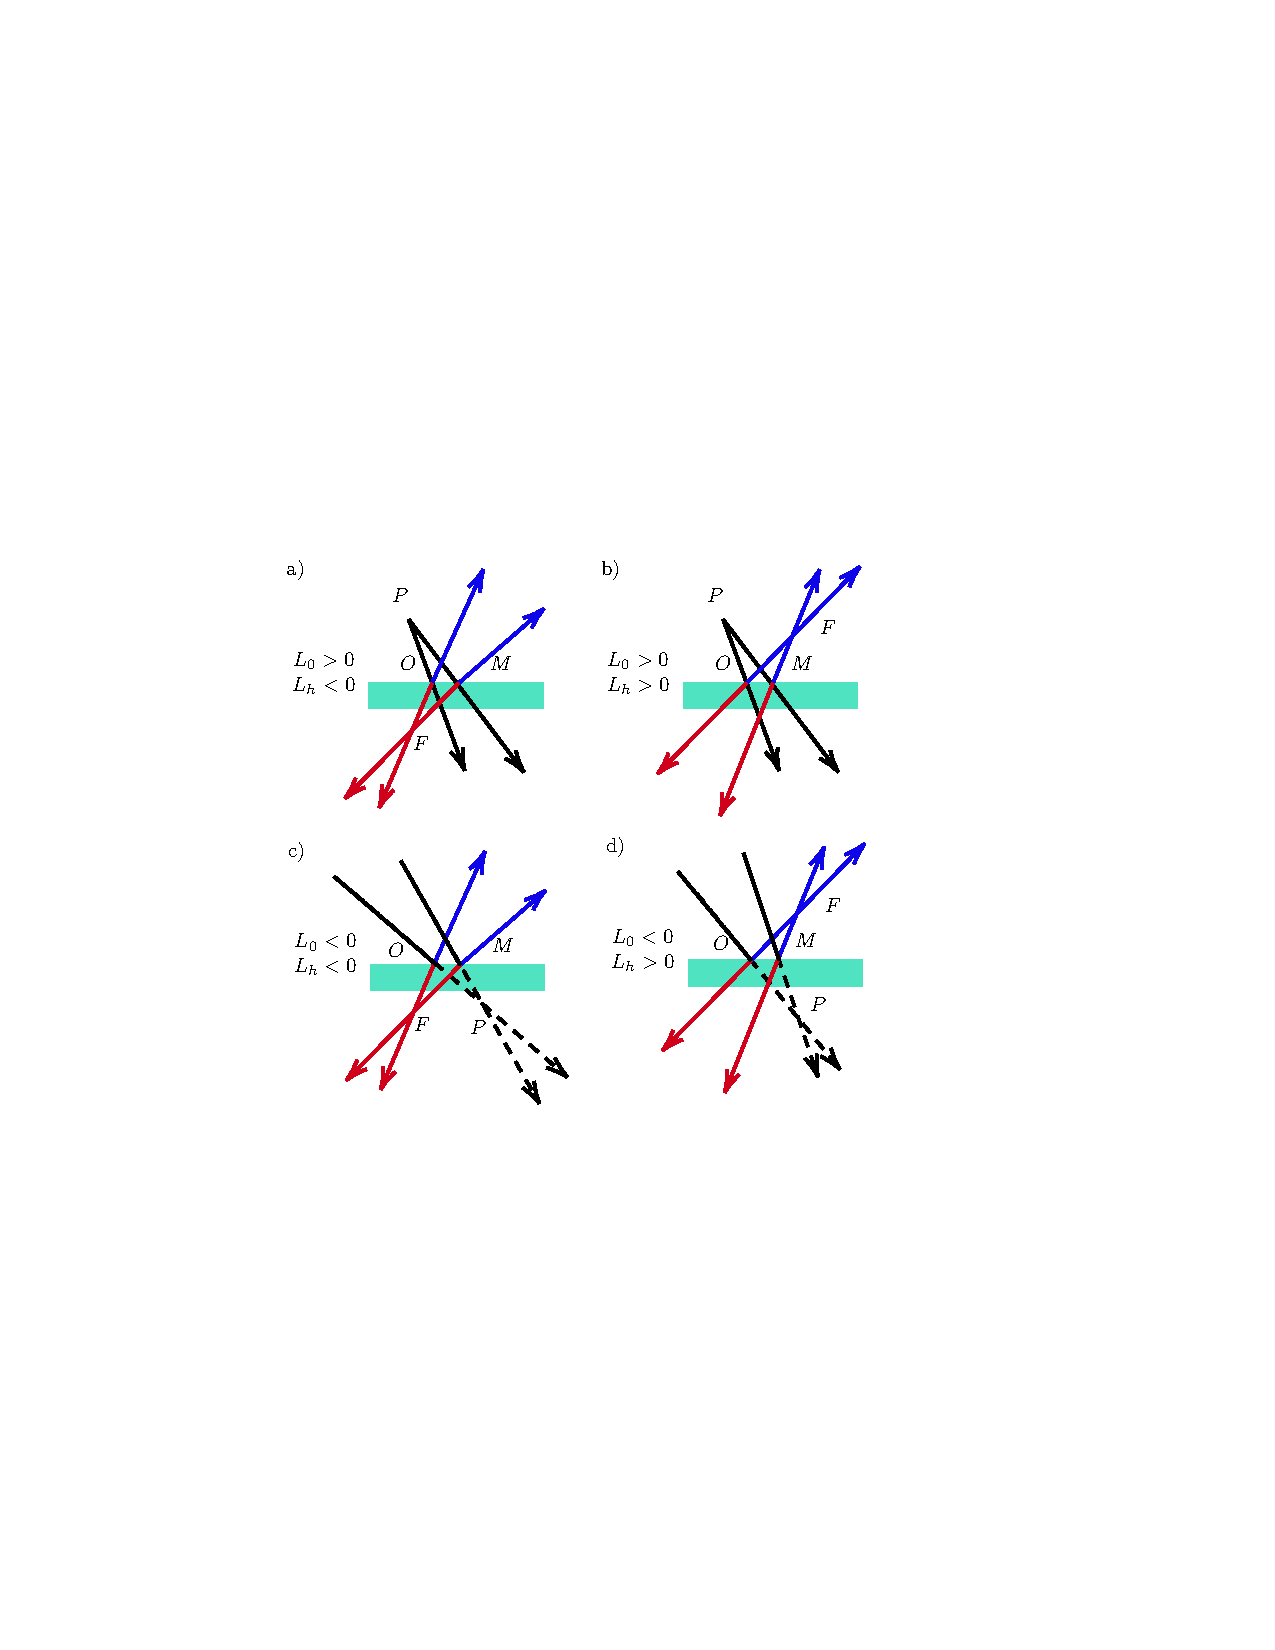
\includegraphics{fig1}
% \end{figure}


\end{document}                    % DO NOT DELETE THIS LINE
%%%%%%%%%%%%%%%%%%%%%%%%%%%%%%%%%%%%%%%%%%%%%%%%%%%%%%%%%%%%%%%%%%%%%%%%%%%%%%
